% Options for packages loaded elsewhere
\PassOptionsToPackage{unicode}{hyperref}
\PassOptionsToPackage{hyphens}{url}
\PassOptionsToPackage{dvipsnames,svgnames,x11names}{xcolor}
%
\documentclass[
  11pt,
]{article}
\usepackage{amsmath,amssymb}
\usepackage{iftex}
\ifPDFTeX
  \usepackage[T1]{fontenc}
  \usepackage[utf8]{inputenc}
  \usepackage{textcomp} % provide euro and other symbols
\else % if luatex or xetex
  \usepackage{unicode-math} % this also loads fontspec
  \defaultfontfeatures{Scale=MatchLowercase}
  \defaultfontfeatures[\rmfamily]{Ligatures=TeX,Scale=1}
\fi
\usepackage{lmodern}
\ifPDFTeX\else
  % xetex/luatex font selection
\fi
% Use upquote if available, for straight quotes in verbatim environments
\IfFileExists{upquote.sty}{\usepackage{upquote}}{}
\IfFileExists{microtype.sty}{% use microtype if available
  \usepackage[]{microtype}
  \UseMicrotypeSet[protrusion]{basicmath} % disable protrusion for tt fonts
}{}
\makeatletter
\@ifundefined{KOMAClassName}{% if non-KOMA class
  \IfFileExists{parskip.sty}{%
    \usepackage{parskip}
  }{% else
    \setlength{\parindent}{0pt}
    \setlength{\parskip}{6pt plus 2pt minus 1pt}}
}{% if KOMA class
  \KOMAoptions{parskip=half}}
\makeatother
\usepackage{xcolor}
\usepackage[margin=24mm]{geometry}
\usepackage{longtable,booktabs,array}
\usepackage{calc} % for calculating minipage widths
% Correct order of tables after \paragraph or \subparagraph
\usepackage{etoolbox}
\makeatletter
\patchcmd\longtable{\par}{\if@noskipsec\mbox{}\fi\par}{}{}
\makeatother
% Allow footnotes in longtable head/foot
\IfFileExists{footnotehyper.sty}{\usepackage{footnotehyper}}{\usepackage{footnote}}
\makesavenoteenv{longtable}
\usepackage{graphicx}
\makeatletter
\def\maxwidth{\ifdim\Gin@nat@width>\linewidth\linewidth\else\Gin@nat@width\fi}
\def\maxheight{\ifdim\Gin@nat@height>\textheight\textheight\else\Gin@nat@height\fi}
\makeatother
% Scale images if necessary, so that they will not overflow the page
% margins by default, and it is still possible to overwrite the defaults
% using explicit options in \includegraphics[width, height, ...]{}
\setkeys{Gin}{width=\maxwidth,height=\maxheight,keepaspectratio}
% Set default figure placement to htbp
\makeatletter
\def\fps@figure{htbp}
\makeatother
\setlength{\emergencystretch}{3em} % prevent overfull lines
\providecommand{\tightlist}{%
  \setlength{\itemsep}{0pt}\setlength{\parskip}{0pt}}
\setcounter{secnumdepth}{5}
\newlength{\cslhangindent}
\setlength{\cslhangindent}{1.5em}
\newlength{\csllabelwidth}
\setlength{\csllabelwidth}{3em}
\newlength{\cslentryspacingunit} % times entry-spacing
\setlength{\cslentryspacingunit}{\parskip}
\newenvironment{CSLReferences}[2] % #1 hanging-ident, #2 entry spacing
 {% don't indent paragraphs
  \setlength{\parindent}{0pt}
  % turn on hanging indent if param 1 is 1
  \ifodd #1
  \let\oldpar\par
  \def\par{\hangindent=\cslhangindent\oldpar}
  \fi
  % set entry spacing
  \setlength{\parskip}{#2\cslentryspacingunit}
 }%
 {}
\usepackage{calc}
\newcommand{\CSLBlock}[1]{#1\hfill\break}
\newcommand{\CSLLeftMargin}[1]{\parbox[t]{\csllabelwidth}{#1}}
\newcommand{\CSLRightInline}[1]{\parbox[t]{\linewidth - \csllabelwidth}{#1}\break}
\newcommand{\CSLIndent}[1]{\hspace{\cslhangindent}#1}
\ifLuaTeX
\usepackage[bidi=basic]{babel}
\else
\usepackage[bidi=default]{babel}
\fi
\babelprovide[main,import]{american}
% get rid of language-specific shorthands (see #6817):
\let\LanguageShortHands\languageshorthands
\def\languageshorthands#1{}
\ifLuaTeX
  \usepackage{selnolig}  % disable illegal ligatures
\fi
\IfFileExists{bookmark.sty}{\usepackage{bookmark}}{\usepackage{hyperref}}
\IfFileExists{xurl.sty}{\usepackage{xurl}}{} % add URL line breaks if available
\urlstyle{same}
\hypersetup{
  pdftitle={Information and Decision Limits in Inferential Predictive Control of a Nonlinear Propylene Glycol Reactor},
  pdfauthor={Walter Yanko de Aragão Brandão},
  pdflang={en-US},
  colorlinks=true,
  linkcolor={Maroon},
  filecolor={Maroon},
  citecolor={Blue},
  urlcolor={Blue},
  pdfcreator={LaTeX via pandoc}}

\title{Information and Decision Limits in Inferential Predictive Control
of a Nonlinear Propylene Glycol Reactor}
\author{Walter Yanko de Aragão Brandão}
\date{20 October 2026}

\begin{document}
\maketitle

\hypertarget{abstract}{%
\section{Abstract}\label{abstract}}

This computational study examines information and decision limits in a
recovered six-state propylene-glycol reactor model. An exact
two-dimensional chemical equivalence class exists with constant species
heat capacities and first-order kinetics. Restoring reciprocal jacket
feedback does not eliminate it. A functional heat-capacity span
characterizes a sufficient surviving ambiguity, while
temperature-dependent property examples test practical separability. The
executed main suite contains 5320 trajectories, with 400
independent-seed confirmation trajectories and 18 grid-sensitivity
checks. At nominal dilution, a two-world initial product separation of
0.8 kmol/m3 yields a worst-world 0.9-hour tracking lower bound of
0.060376 kmol h/m3. Finite-grid decision conflict is positive in 51 of
80 examined cases. Incremental ambiguity-control mean gains were 0.63\%
and 0.66\%, with paired confidence intervals including zero; predictor
sharing reduced IAE by 39.91\% versus estimator-only adaptation. These
outcomes do not establish superiority over all continuous NMPC designs.
The physical alternatives remain uncalibrated and historical ICAC scalar
results were not independently replayed. Accordingly this is a partial
research manuscript, not a completed submission-ready validation. \#
Introduction

Inferential quality control relies on the information carried by
measured variables and on the predictions used to choose actions. A
smaller concentration RMSE need not reduce closed-loop loss. This study
audits a six-state propylene-glycol CSTR before evaluating additional
estimation or control complexity. Two questions are separated: whether
temperature-only measurements leave a demonstrable chemical ambiguity,
and whether explicitly representing that ambiguity improves control
against equally informed comparators.

The recovered internal ICAC study already reported calorimetrically
indistinguishable states and decision conflicts. Its numerical
percentages are historical evidence, not reproduced findings of this
campaign. The current branch and complete raw ICAC archive were
unavailable. This manuscript therefore reports an independent
computational core, with remaining publication requirements explicitly
identified.

\hypertarget{related-work}{%
\section{Related work}\label{related-work}}

Nonlinear observability and identifiability theory distinguish
information loss from numerical estimation difficulty (Hermann and
Krener 1977; Villaverde, Barreiro, and Papachristodoulou 2016). Reactor
concentration ambiguity is not new: nonmonotone kinetic examples already
motivate detectable output-feedback designs (Schaum et al. 2007).
Empirical trajectory methods can reveal weak directions without proving
a global structural result (Lall, Marsden, and Glavaski 2002).

Constrained MHE and output-feedback MPC have established assumptions and
stability frameworks (Rao, Rawlings, and Mayne 2003; Rawlings, Mayne,
and Diehl 2017). Regret-optimal measurement feedback has a different
benchmark in existing linear-control results (Goel and Hassibi 2021).
Decision-aware prediction and dual control also precede this study
(Elmachtoub and Grigas 2022; Klenske and Hennig 2016). Recent
belief-space approaches treat input-dependent observations or latent
parameter risk (Cao et al. 2026; Enwerem, Baras, and Belta 2026); those
preprints do not establish reactor performance. The present candidate
contribution is a traced, model-specific heat-capacity classification
and its connection to finite-horizon decision experiments.

\hypertarget{physical-process-model}{%
\section{Physical process model}\label{physical-process-model}}

The historical source is Brandão's dissertation and recovered executable
MATLAB model (Brandao 2019). The reaction is A+B to C, with methanol M
treated as inert, constant reactor volume and a level-controlled outlet.
Concentrations are kmol/m3, temperatures K, time h and heat kJ. Let
\[v=F_A/\rho_A+F_B/\rho_B+F_M/\rho_M,\quad D=v/V,\quad
r=k_0\exp[-E/(R(T+0.183333333333))]C_A.\] The balances are
\[\dot C_A=F_A/V-DC_A-r,\qquad \dot C_B=F_B/V-DC_B-r,\]
\[\dot C_C=-DC_C+r,\qquad\dot C_M=F_M/V-DC_M.\] With
\(W=\sum_i c_{p,i}C_i\) and \(F_{cp}=F_Ac_{p,A}+F_Bc_{p,B}+F_Mc_{p,M}\),
\[Q=m_wc_{p,B}(T_a-T)[1-e^{-UA/(m_wc_{p,B})}],\]
\[\dot T=\frac{Q+F_{cp}(T_0-T)-\Delta H_r rV}{VW},\qquad
\dot T_t=\frac{m_wc_{p,B}(T_a-T_t)-Q}{\rho_BV_tc_{p,B}}.\] Only
\(T,T_t\) are measured. The sole optimized input is \(m_w=q\,453.59237\)
kmol/h; current feeds are known, future disturbances are not. The
historical asymmetry is retained: \(T_t\) does not enter \(Q\).

The executable enthalpy is -83736 kJ/kmol; the dissertation table
instead lists -91556.90. The archive's rounded imperial conversion and
Fahrenheit offset are preserved as benchmark conventions, not new
physical findings. The public Fogler example also contains a temperature
correction to reaction heat, but at different operating conditions
(Fogler, n.d.). It does not justify replacing the dissertation constants
without calibration.

A related teaching case uses excess-water first-order kinetics and
models the liquid as nonideal (Chan and Seider 2004). This supports
retaining the historical kinetic approximation as a benchmark, while
showing why ideal-mixture calorimetry alone cannot establish physical
equivalence in a real reactor.

The constant-volume benchmark computes volumetric outflow from feed
densities but does not impose a composition-dependent equation of state
or partial-molar-volume closure on each candidate inventory. Positivity
therefore establishes model admissibility, not full physical
admissibility of a liquid mixture. Additional exact composition/volume
constraints would intersect the invisible subspace and can reduce it;
they require independent physical data. Reaction volume change and
nonideal mixture enthalpy remain outside the reconciliations tested
here.

\hypertarget{explicit-physical-alternatives}{%
\subsection{Explicit physical
alternatives}\label{explicit-physical-alternatives}}

M1H adds Kirchhoff consistency:
\(\Delta H_r(T)=\Delta H_r(T_r)+\int_{T_r}^T(c_{p,C}-c_{p,A}-c_{p,B})\,d\theta\),
with the historical enthalpy assumed to refer to nominal
\(T_r=332.333618020\) K. This reference is not independently known. M1J
also uses \(Q=G(T_t-T)\) and the existing jacket storage balance. The
conductance \(G=m_{w0}c_{p,B}[\exp(UA/(m_{w0}c_{p,B}))-1]\) matches
nominal stationary cooling, rather than asserting that coil UA and
mixed-jacket conductance are identical.

M2L and M2Q use \(c_{p,i}(T)=a_i+b_i(T-T_r)+c_i(T-T_r)^2\), where
\(a_i\) are historical capacities. Relative slopes are
(0.0015,0.0002,0.0025,0.0010) per K; relative curvatures are
(0.000010,0.000002,0.000016,-0.000003) per K squared. M2L sets all
curvatures to zero. Feed sensible enthalpies and reaction enthalpy are
integrated consistently. These are synthetic sensitivity models. They
are not calibrated physical-property correlations, and no one is called
the validated M1 of the original research request.

\hypertarget{estimation-and-control-architectures}{%
\section{Estimation and control
architectures}\label{estimation-and-control-architectures}}

B1 uses a six-state UKF and nominal predictive model. B2\_estimator
augments the UKF with log kinetic and heat-transfer factors, while
retaining a nominal predictor. B2\_both shares the same estimated
factors with the predictor. Neither receives true parameters. B0 is a
documented fixed PI using the inferred product, with gains 4 and 2 and
antiwindup. It is not a reproduced optimally tuned historical cascade.

B3\_assumed\_inventory imposes nominal initial inventories.
B3\_known\_inventory receives exact initial inventories once, and
therefore has additional information. The reduced state is
\((C_C,T,T_t)\); conserved totals follow their feed/dilution equations.
B4 is a deterministic six-step MHE with an approximate arrival prior, no
process-noise decision variables and 18 function-evaluation budget. B5
uses the true current state only as a diagnostic oracle, with nominal
predictive parameters.

P1 evaluates mean cost of three representatives. P2 minimizes their
largest regret. P3 combines this rule with causal parameter adaptation.
P4 uses the robust action when representative first actions differ by at
least 0.2 nominal coolant units; otherwise it applies the adapted
nominal policy. The representatives are a UKF point and calorimetrically
compensated product offsets of plus/minus \(0.4e^{-\int Ddt}\). They are
not a certified set enclosure or a posterior sample; a finite set cannot
represent every possible physical state.

P5 variants retain nominal control and add chemical samples: initial
only; four periodic samples; event-triggered with quota four; three-step
delay; higher measurement noise; or up to eight frequent samples.
Immediate product samples have standard deviation 0.03 kmol/m3, the
noisy case 0.15. Delayed innovations are transported approximately with
dilution and an explicit variance increment; a full out-of-sequence
smoother is not implemented. Event requests use available belief width
and previous action disagreement, never future measurements.

The standard policy enumerates at most 25 two-block sequences: the first
action lasts three steps and the second eleven. Candidate increments are
five equally spaced values from -0.4 to 0.4. All methods in each
scenario share \(0.05\le q\le3\) and step change at most 0.4; saturation
cases use the same lower maximum 1.3 for all methods. The sampled
constraint is \(T\le344.261111\) K. A no-common-feasible-plan event
triggers an explicitly logged least-violation fallback; no safety
guarantee is inferred.

The dimensionless horizon cost is
\[J=\sum_{j=1}^{14}\left[0.8\left(\frac{C_{C,j}-r_k}{2.295764605}\right)^2+
1000\left(\frac{\max(T_j-344.261111,0)}{160/1.8}\right)^2\right]
+0.2[(q_1-q_{\rm prev})^2+(q_2-q_1)^2].\] This cost is not IAE.
B1\_continuous additionally optimizes the same two-block problem using
SLSQP, initialized by the grid solution; it is a local numerical
comparator, not the full historical 57-step/six-move NMPC.

\hypertarget{experimental-methodology}{%
\section{Experimental methodology}\label{experimental-methodology}}

The frozen protocol specifies 14 scenarios, 19 methods and 20 paired
seeds per combination. Sixty intervals of 0.015 h give 0.9 h per
trajectory. Scenarios include nominal operation, reference changes,
kinetic and heat-transfer errors, signed inventory ambiguity, current
feed disturbances, heat-capacity error, correlated noise, sensor
dropout, saturation, combined perturbations, a state outside the
representative prior and an unreachable reference. Hypothetical
structural-physics variants are analyzed separately from the M0 control
benchmark.

The UKF prior standard deviations are (0.15,0.8,0.4,0.3,0.5,0.5);
process covariance diagonal is (2e-6,2e-5,2e-6,1e-7,0.015,0.006).
Temperature-noise standard deviations are (1.385,1.062)/1.8 K. Adaptive
log factors have initial variance 0.15 squared, process variance 1e-5
and bounds {[}-0.5,0.5{]}. UKF alpha=0.5 and beta=2. No tuning uses
held-out outcomes.

Main seeds are 4100--4119. Confirmation seeds 8100--8119 address four
declared scenarios and five relevant methods. Validation seeds 101--103
evaluate a denser grid. Development seed 11 is used for short runtime
checks. Noise trajectories are matched across methods. Bootstrap units
are paired seeds; finite-suite means first average each seed across the
fixed scenario list. Uncertainty describes this finite suite, not an
industrial population. Three primary contrasts receive Holm adjustment;
other contrasts remain exploratory.

The plant uses RK4 with 12 substeps, compared against SciPy DOP853 with
rtol 2e-11 and atol 1e-12. Prediction uses three substeps; filtering
uses four. Physical state trajectories are not clipped. Filter
positivity and covariance repairs are logged. Scalar metrics are
independently recalculated from saved trajectories. Timing is from a
Linux hosted CPU, without evidence of performance on the target Ryzen
system.

\hypertarget{parameters-and-initial-condition}{%
\section{Parameters and initial
condition}\label{parameters-and-initial-condition}}

\begin{longtable}[]{@{}lll@{}}
\toprule\noalign{}
Parameter & Value & Unit \\
\midrule\noalign{}
\endhead
\bottomrule\noalign{}
\endlastfoot
V & 1.89183 & m3 \\
Vt & 1.10011 & m3 \\
UA & 30385.6 & kJ/(h K) \\
CpA & 146.538 & kJ/(kmol K) \\
CpB & 75.3624 & kJ/(kmol K) \\
CpC & 192.593 & kJ/(kmol K) \\
CpM & 81.6426 & kJ/(kmol K) \\
E & 75362.4 & kJ/kmol \\
R & 8.31917 & kJ/(kmol K) \\
k0 & 1.696e+13 & 1/h \\
DeltaH & -83736 & kJ/kmol \\
FA & 36.2874 & kmol/h \\
FB & 453.592 & kmol/h \\
FM & 45.3592 & kmol/h \\
mw0 & 453.592 & kmol/h \\
T0 & 297.039 & K \\
Ta & 288.706 & K \\
\end{longtable}

Nominal equilibrium: 0.607024732, 33.989102107, 2.295764605,
3.628486671, 332.333618020, 314.397585330.

\hypertarget{mathematical-scope-and-proofs}{%
\section{Mathematical scope and
proofs}\label{mathematical-scope-and-proofs}}

All statements below concern the stated model class, not an
experimentally identified industrial reactor. Time is in hours. All
worlds share the same known feed histories, parameters, reference,
actuator constraints and initial measured temperatures. Initial chemical
states range over an open positive domain admitted by the six-state
benchmark. This does not impose a separately validated liquid equation
of state. If additional exact admissibility constraints are imposed, the
constructed equivalence class must be intersected with them; its quoted
dimension need not survive. Solutions are unique up to the considered
finite horizon and remain in that set. Inputs can depend causally on
measured temperatures. Exact information statements use noiseless
measurements or a coupling with the same additive sensor-noise
realization.

\hypertarget{proposition-1-a-calorimetric-equivalence-class}{%
\subsection{Proposition 1: a calorimetric equivalence
class}\label{proposition-1-a-calorimetric-equivalence-class}}

Let the four species obey \(\dot c=F/V-D(t)c+\nu r\), with
\(\nu=(-1,-1,1,0)^T\) and \(r=k(T)C_A\). Suppose the thermal dynamics
depend on composition only through \(C_A\) and
\(W(T,c)=\sum_i c_{p,i}(T)C_i\). Heat exchange can be any locally
Lipschitz function of \(T,T_t,u\) independent of the remaining chemical
coordinates. Reaction enthalpy can depend on temperature, consistently
or otherwise, without changing this statement.

For constant heat capacities, two initial states satisfying
\[\delta C_A=0,\quad\delta T=\delta T_t=0,\qquad
c_{p,B}\delta C_B+c_{p,C}\delta C_C+c_{p,M}\delta C_M=0\] generate
identical temperatures for every common admissible input, for as long as
both trajectories exist in the physical domain. The chemical differences
are \[\delta c(t)=e^{-\int_0^tD(s)\,ds}\delta c(0).\]

Proof. Equal \(C_A,T\) imply equal reaction rates. Subtraction of the
species balances then gives homogeneous dilution for the remaining
differences. Their calorimetric combination stays zero, so both thermal
derivatives agree. Uniqueness closes the argument. Under causal
feedback, equal histories imply equal next actions, and uniqueness
continues the equality. There are two independent chemical directions in
this kernel. Thus the six free states cannot be locally reconstructed in
full. The observable quotient has at most four coordinates
\((C_A,W,T,T_t)\). This is a sufficient construction of
indistinguishability, not a claim that all indistinguishable pairs have
this form.

This result survives restoring reciprocal heat transfer between jacket
and reactor. Therefore the absence of jacket feedback is not, by itself,
the cause of the two-dimensional composition ambiguity.

\hypertarget{proposition-1b-functional-heat-capacity-rank}{%
\subsection{Proposition 1b: functional heat-capacity
rank}\label{proposition-1b-functional-heat-capacity-rank}}

Define the linear space
\[\mathcal S=\operatorname{span}\{(c_{p,B}(T),c_{p,C}(T),c_{p,M}(T)):T\in\mathcal I\}.\]
Every difference with \(\delta C_A=0\) and
\((\delta C_B,\delta C_C,\delta C_M)\in\mathcal S^\perp\) satisfies the
same construction. Its dimension is \(3-\dim\mathcal S\).

Proof. Its thermal capacity difference vanishes at every temperature in
\(\mathcal I\). The species differences all acquire the same scalar
dilution factor. The preceding proof applies unchanged, including
temperature-dependent reaction enthalpy and feed sensible enthalpies.
For constant Cp, rank is one. For species-wise affine Cp(T), rank is at
most two, leaving at least one invisible direction. For independent
quadratic Cp functions, this particular kernel can disappear. The
absence of this kernel is NOT a proof of complete nonlinear
observability: other symmetries, singular operating states and poor
sensitivity may remain.

A useful sensor-design consequence follows. A scalar chemical
measurement \(a^Tc\) resolves product on a given equivalence class only
if \[\ker(a^T|_{\mathcal N})\subseteq\ker(e_C^T|_{\mathcal N}),\] where
\(\mathcal N\) is the invisible chemical subspace. Measuring \(C_C\)
directly satisfies this requirement, while an arbitrary additional
concentration need not. Known \(C_A+C_C\) also determines product once
\(C_A\) is identified, but its initial value is additional information.

\hypertarget{proposition-1c-a-bad-constant-input-and-a-local-quotient-test}{%
\subsection{Proposition 1c: a bad constant input and a local quotient
test}\label{proposition-1c-a-bad-constant-input-and-a-local-quotient-test}}

For M0 with constant inputs, write \(A=C_A\), \(W=\sum c_{p,i}C_i\),
\(q=F_A/V\), \(c=F_{cp}/V\), \(n=c_{p,C}-c_{p,A}-c_{p,B}\),
\(a(T)=[Q(T)+F_{cp}(T_0-T)]/V\) and \(b(T)=-\Delta H_r k(T)\). Then
\(\dot A=q-(D+k)A,\quad\dot W=c-DW+nkA,\quad g=\dot T=(a+bA)/W.\) At a
chemical/thermal stationary point with \(\dot A=0\) and \(a+bA=0\),
arbitrary sufficiently small perturbations of B, C and M leave A and
both temperatures constant under this same fixed input. They merely
change W and decay with dilution. Thus three chemical directions are
invisible under this particular unexcited experiment, although only two
belong to the preceding all-input calorimetric family. Excitation can
distinguish the extra direction. This is a property of a fixed input
experiment, not a claim of a three-dimensional all-input symmetry.

A useful sufficient local test uses the gradients of
\(T,T_t,L_fT,L_f^2T\) on the quotient \((A,W,T,T_t)\). The relevant
two-by-two minor for \((A,W)\) is
\(\det\begin{bmatrix}g_A&g_W\\(L_fg)_A&(L_fg)_W\end{bmatrix} =-\frac{b[bq+(D+k)a]}{W^3} +\frac{(a+bA)[-ba_T+bc+ab_T-ank]}{W^4}.\)
This follows by differentiating
\(L_fg=\frac{bq+Da-bkA}{W} +\frac{(a+bA)(a_T+b_TA-c-nkA)}{W^2}.\) A
nonzero minor is sufficient for rank four of this local quotient
observability test. It vanishes at the nominal equilibrium under the
constant input. A zero value alone does not prove unobservability; the
explicit invariant-trajectory construction above proves the special
equilibrium case. The six-state model still has rank at most four under
the all-input symmetry. Numerical arbitrary-precision evaluations are
supporting local computations, not a global rank theorem.

\hypertarget{proposition-2-estimation-and-tracking-bounds}{%
\subsection{Proposition 2: estimation and tracking
bounds}\label{proposition-2-estimation-and-tracking-bounds}}

Let two possible product concentrations at time \(t\) have separation
\(\Delta(t)\). Any estimator based on their common information has the
same output in both worlds, hence
\[\max_i|\hat C_C(t)-C_C^{(i)}(t)|\geq\Delta(t)/2.\] The proof is the
triangle inequality. The midpoint attains the bound if precisely those
two values are the only possibilities, so the two-point bound is sharp
under that information model.

The same inequality holds with a common tracking reference in place of
the estimate. Integrating gives a different, trajectory-level statement:
\[\max_i\operatorname{IAE}_i(H)\geq\frac12\int_0^H\Delta(t)\,dt.\] For
constant dilution and initial separation \(\Delta_0\), the right-hand
side is \(\Delta_0(1-e^{-DH})/(2D)\). This is a bound on worst-case
tracking error, not on regret relative to a state-informed oracle. The
oracle may itself have unavoidable transient tracking loss. Decay of
these bounds by dilution is physical replacement of the unknown initial
inventory, not information supplied by the sensors.

For a fixed open-loop input and two Gaussian observation records with
the same known covariance \(\Sigma\), their KL divergence is
\(\frac12(\mu_1-\mu_2)^T\Sigma^{-1}(\mu_1-\mu_2)\). A two-world expected
absolute estimation-risk bound is \(\Delta(1-\mathrm{TV})/2\); using
Pinsker gives the nonnegative bound
\(\Delta\max(0,1-\sqrt{\mathrm{KL}/2})/2\). This does not apply
unchanged to adaptive noisy feedback with action-dependent product
separation. The present campaign does not claim an industrial stochastic
lower bound from this formula.

\hypertarget{proposition-3-state-ambiguity-versus-decision-conflict}{%
\subsection{Proposition 3: state ambiguity versus decision
conflict}\label{proposition-3-state-ambiguity-versus-decision-conflict}}

Let a finite set of indistinguishable worlds have continuous costs
\(J_i\) on a common nonempty compact feasible action-sequence set
\(\mathcal U\). Let \(J_i^*=\min_{u\in\mathcal U}J_i(u)\). Define
\[\mathcal R^*=\min_{u\in\mathcal U}\max_i[J_i(u)-J_i^*].\] Then
\(\mathcal R^*=0\) if and only if the worlds' minimizing sets have a
common point. Otherwise \(\mathcal R^*>0\).

Proof. Regrets are nonnegative. A common minimizer makes every regret
zero. Conversely, continuity and compactness give a minimizer of the
maximum regret; if its value is zero, that point minimizes every cost.
Disjoint minimizers therefore imply a strictly positive attained value.
Large chemical separation can coexist with zero decision regret when all
worlds prefer the same action, including common actuator saturation.

If world-specific feasibility sets differ, evaluate individual optima in
their declared sets and the robust decision in their intersection. An
empty intersection is infeasibility, not finite regret. Numerical
results explicitly mark absent common feasible candidates.

\hypertarget{proposition-3b-when-representing-ambiguity-cannot-change-the-expected-cost-action}{%
\subsection{Proposition 3b: when representing ambiguity cannot change
the expected-cost
action}\label{proposition-3b-when-representing-ambiguity-cannot-change-the-expected-cost-action}}

For the exact PG twins with the same known feed history, coolant flow
does not change the dilution rate. Let the possible products under any
common plan be \(C_C(t;u,\delta)=C_C(t;u,0)+d(t)\delta\), with
\(d(t)=e^{-\int_0^tD(s)ds}\) independent of the optimized coolant plan.
Suppose the distribution over offsets has zero mean, all representatives
remain physically admissible, the feasibility constraints depend only on
their common thermal states and actions, and the tracking cost is a
fixed weighted sum of squared product errors plus common thermal and
actuation costs. Then
\(\mathbb E_\delta J_\delta(u)=J_0(u)+\mathbb E[\delta^2]\sum_j w_jd(t_j)^2,\)
where the final term is independent of \(u\). Therefore nominal and
expected-cost optimization have exactly the same minimizing action set.
The result holds for both finite and continuous action classes under
these assumptions.

Proof. Expand each squared error and average. The cross term vanishes by
the zero-mean offset, while all other costs and constraints are shared.
This is a certainty-equivalence special case, not a universal robustness
theorem. Nonquadratic losses, action-dependent dilution, asymmetrically
truncated beliefs, state-dependent physical constraints or a changed
information policy can invalidate it. In the implemented symmetric
three-representative P1 experiment it predicts a null control benefit,
apart from admissibility exclusions and numerical tie handling. This is
a falsification of any claim that merely including those symmetric
worlds must improve this quadratic NMPC.

\hypertarget{proposition-4-a-conditional-quantitative-regret-bound}{%
\subsection{Proposition 4: a conditional quantitative regret
bound}\label{proposition-4-a-conditional-quantitative-regret-bound}}

If two costs are \(\mu\)-strongly convex on the same convex action set
and have respective minimizers \(u_1^*,u_2^*\), then
\[\mathcal R^*\geq\frac{\mu}{8}\|u_1^*-u_2^*\|^2.\] Strong convexity and
first-order optimality yield
\(J_i(u)-J_i(u_i^*)\geq\mu\|u-u_i^*\|^2/2\). At least one distance is at
least half the distance between the minimizers, proving the bound.
Convexity also prevents improvement by randomizing actions when the
criterion is maximum expected cost. These convexity conditions are NOT
established for the nonlinear PG optimization. Accordingly no numerical
PG regret is described as certified by this bound.

For exact indistinguishability over a whole horizon and deterministic
noiseless causal policies whose realizable sequences belong to
\(\mathcal U\), every policy realizes a common sequence. Its maximum
regret is at least the minimax value over \(\mathcal U\). A finite
candidate grid supplies an exact result only within that grid. If the
per-world oracle costs are held fixed at their continuous optima,
restricting the decision set gives an upper bound on the continuous
minimax value. Here both the decisions and the per-world oracle optima
are restricted to the grid. Consequently the reported value has no
general one-sided bound relative to continuous minimax regret. It is not
a lower bound valid for all physical controllers. If future measurements
can distinguish the worlds, open-loop sequence regret cannot be
substituted for the value of an optimal adaptive policy.

\hypertarget{known-scope-versus-possible-contribution}{%
\subsection{Known scope versus possible
contribution}\label{known-scope-versus-possible-contribution}}

Observability, detectability, two-point risk bounds, minimax regret and
decision-aware estimation are established concepts. The proofs above are
elementary specializations and should not be advertised as a new
universal control law. The candidate case-specific contribution is the
functional-Cp classification, its application to a traced PG model, and
an audit connecting physical closure, distinguishability, chemical
sampling and decision cost. A comprehensive novelty review and
calibrated physical data are still needed.

\hypertarget{numerical-results}{%
\section{Numerical results}\label{numerical-results}}

Completed execution and paired comparisons are shown below. Positive
improvement favors the first method. The finite-suite CI resamples 20
paired seed clusters and is conditional on the chosen scenarios.

\begin{longtable}[]{@{}
  >{\raggedright\arraybackslash}p{(\columnwidth - 12\tabcolsep) * \real{0.1429}}
  >{\raggedright\arraybackslash}p{(\columnwidth - 12\tabcolsep) * \real{0.1429}}
  >{\raggedright\arraybackslash}p{(\columnwidth - 12\tabcolsep) * \real{0.1429}}
  >{\raggedright\arraybackslash}p{(\columnwidth - 12\tabcolsep) * \real{0.1429}}
  >{\raggedright\arraybackslash}p{(\columnwidth - 12\tabcolsep) * \real{0.1429}}
  >{\raggedright\arraybackslash}p{(\columnwidth - 12\tabcolsep) * \real{0.1429}}
  >{\raggedright\arraybackslash}p{(\columnwidth - 12\tabcolsep) * \real{0.1429}}@{}}
\toprule\noalign{}
\begin{minipage}[b]{\linewidth}\raggedright
candidate
\end{minipage} & \begin{minipage}[b]{\linewidth}\raggedright
baseline
\end{minipage} & \begin{minipage}[b]{\linewidth}\raggedright
percent\_improvement
\end{minipage} & \begin{minipage}[b]{\linewidth}\raggedright
mean\_improvement
\end{minipage} & \begin{minipage}[b]{\linewidth}\raggedright
ci95\_low
\end{minipage} & \begin{minipage}[b]{\linewidth}\raggedright
ci95\_high
\end{minipage} & \begin{minipage}[b]{\linewidth}\raggedright
p\_holm\_primary
\end{minipage} \\
\midrule\noalign{}
\endhead
\bottomrule\noalign{}
\endlastfoot
P2\_regret & B1\_ukf & 0.634593 & 0.000850102 & -0.00100823 & 0.00283537
& 0.418569 \\
P3\_adaptive\_regret & B2\_both & 0.657212 & 0.000578973 & -0.000207131
& 0.00145957 & 0.418569 \\
B2\_both & B2\_estimator & 39.912 & 0.0585153 & 0.0565261 & 0.0604609 &
3.11056e-22 \\
\end{longtable}

\hypertarget{model-and-information-experiments}{%
\subsection{Model and information
experiments}\label{model-and-information-experiments}}

\begin{longtable}[]{@{}lll@{}}
\toprule\noalign{}
variant & max\_thermal\_difference\_K & max\_product\_decay\_error \\
\midrule\noalign{}
\endhead
\bottomrule\noalign{}
\endlastfoot
M0\_historical & 5.68434e-14 & 5.8647e-12 \\
M1H\_Kirchhoff\_hypothesis & 0 & 5.86337e-12 \\
M1J\_mixed\_jacket\_hypothesis & 0 & 5.86159e-12 \\
M2L\_linear\_cp\_hypothesis & 1.03074e-05 & 3.37664e-07 \\
M2Q\_quadratic\_cp\_hypothesis & 9.3374e-06 & 3.16407e-07 \\
\end{longtable}

\hypertarget{input-dependent-local-rank-and-surviving-affine-property-twins}{%
\subsection{Input-dependent local rank and surviving affine-property
twins}\label{input-dependent-local-rank-and-surviving-affine-property-twins}}

\begin{longtable}[]{@{}llll@{}}
\toprule\noalign{}
T & determinant & derivative\_check\_error & sufficient\_rank4 \\
\midrule\noalign{}
\endhead
\bottomrule\noalign{}
\endlastfoot
315 & 3.14609 & 3.19241e-58 & True \\
325 & 60.5759 & 1.07534e-57 & True \\
332.334 & 8.10924e-58 & 1.84845e-57 & False \\
340 & -893.845 & 5.2572e-57 & True \\
348 & -5623.79 & 4.46066e-57 & True \\
\end{longtable}

\begin{longtable}[]{@{}
  >{\raggedright\arraybackslash}p{(\columnwidth - 8\tabcolsep) * \real{0.2000}}
  >{\raggedright\arraybackslash}p{(\columnwidth - 8\tabcolsep) * \real{0.2000}}
  >{\raggedright\arraybackslash}p{(\columnwidth - 8\tabcolsep) * \real{0.2000}}
  >{\raggedright\arraybackslash}p{(\columnwidth - 8\tabcolsep) * \real{0.2000}}
  >{\raggedright\arraybackslash}p{(\columnwidth - 8\tabcolsep) * \real{0.2000}}@{}}
\toprule\noalign{}
\begin{minipage}[b]{\linewidth}\raggedright
constant\_input\_max\_thermal\_difference
\end{minipage} & \begin{minipage}[b]{\linewidth}\raggedright
excited\_uncompensated\_max\_thermal\_difference
\end{minipage} & \begin{minipage}[b]{\linewidth}\raggedright
affine\_kernel\_max\_thermal\_difference
\end{minipage} & \begin{minipage}[b]{\linewidth}\raggedright
affine\_functional\_rank
\end{minipage} & \begin{minipage}[b]{\linewidth}\raggedright
quadratic\_functional\_rank
\end{minipage} \\
\midrule\noalign{}
\endhead
\bottomrule\noalign{}
\endlastfoot
0 & 0.037972 & 0 & 2 & 3 \\
\end{longtable}

\hypertarget{selected-absolute-metrics}{%
\subsection{Selected absolute metrics}\label{selected-absolute-metrics}}

\begin{longtable}[]{@{}
  >{\raggedright\arraybackslash}p{(\columnwidth - 10\tabcolsep) * \real{0.1667}}
  >{\raggedright\arraybackslash}p{(\columnwidth - 10\tabcolsep) * \real{0.1667}}
  >{\raggedright\arraybackslash}p{(\columnwidth - 10\tabcolsep) * \real{0.1667}}
  >{\raggedright\arraybackslash}p{(\columnwidth - 10\tabcolsep) * \real{0.1667}}
  >{\raggedright\arraybackslash}p{(\columnwidth - 10\tabcolsep) * \real{0.1667}}
  >{\raggedright\arraybackslash}p{(\columnwidth - 10\tabcolsep) * \real{0.1667}}@{}}
\toprule\noalign{}
\begin{minipage}[b]{\linewidth}\raggedright
scenario
\end{minipage} & \begin{minipage}[b]{\linewidth}\raggedright
method
\end{minipage} & \begin{minipage}[b]{\linewidth}\raggedright
IAE
\end{minipage} & \begin{minipage}[b]{\linewidth}\raggedright
RMSE\_CC
\end{minipage} & \begin{minipage}[b]{\linewidth}\raggedright
Tmax
\end{minipage} & \begin{minipage}[b]{\linewidth}\raggedright
fallback
\end{minipage} \\
\midrule\noalign{}
\endhead
\bottomrule\noalign{}
\endlastfoot
combined & B1\_continuous & 0.220454 & 0.130548 & 332.334 & 0 \\
combined & B1\_ukf & 0.230553 & 0.130567 & 332.353 & 0 \\
combined & B2\_both & 0.0797465 & 0.0764126 & 337.065 & 0 \\
combined & B2\_estimator & 0.253608 & 0.077038 & 332.334 & 0 \\
combined & B4\_mhe & 0.191722 & 0.118114 & 332.58 & 0 \\
combined & P2\_regret & 0.232497 & 0.130859 & 332.334 & 0 \\
combined & P3\_adaptive\_regret & 0.078689 & 0.0763533 & 337.167 & 0 \\
inventory\_plus & B1\_continuous & 0.0615694 & 0.122312 & 332.612 & 0 \\
inventory\_plus & B1\_ukf & 0.0603865 & 0.122254 & 332.442 & 0 \\
inventory\_plus & B2\_both & 0.0617974 & 0.122231 & 332.925 & 0 \\
inventory\_plus & B2\_estimator & 0.060544 & 0.122043 & 332.439 & 0 \\
inventory\_plus & B4\_mhe & 0.0602121 & 0.122743 & 332.429 & 0 \\
inventory\_plus & P2\_regret & 0.059559 & 0.122162 & 332.372 & 0 \\
inventory\_plus & P3\_adaptive\_regret & 0.0626549 & 0.122186 & 332.894
& 0 \\
kinetic & B1\_continuous & 0.16428 & 0.081211 & 332.334 & 0 \\
kinetic & B1\_ukf & 0.192631 & 0.0839044 & 332.334 & 0 \\
kinetic & B2\_both & 0.0448606 & 0.0153278 & 333.993 & 0 \\
kinetic & B2\_estimator & 0.234377 & 0.0168838 & 332.334 & 0 \\
kinetic & B4\_mhe & 0.17914 & 0.0732316 & 332.334 & 0 \\
kinetic & P2\_regret & 0.183597 & 0.0835791 & 332.334 & 0 \\
kinetic & P3\_adaptive\_regret & 0.0437234 & 0.0153134 & 333.85 & 0 \\
nominal & B1\_continuous & 0.00323946 & 0.0112444 & 332.612 & 0 \\
nominal & B1\_ukf & 0.00164715 & 0.01124 & 332.442 & 0 \\
nominal & B2\_both & 0.00751547 & 0.0148704 & 332.925 & 0 \\
nominal & B2\_estimator & 0.00143415 & 0.0148619 & 332.439 & 0 \\
nominal & B4\_mhe & 0.00163409 & 0.0120908 & 332.429 & 0 \\
nominal & P2\_regret & 0.00144464 & 0.0112486 & 332.372 & 0 \\
nominal & P3\_adaptive\_regret & 0.00606505 & 0.014836 & 332.894 & 0 \\
\end{longtable}

\hypertarget{independent-confirmation}{%
\subsection{Independent confirmation}\label{independent-confirmation}}

\begin{longtable}[]{@{}lllll@{}}
\toprule\noalign{}
candidate & baseline & percent\_improvement & ci95\_low & ci95\_high \\
\midrule\noalign{}
\endhead
\bottomrule\noalign{}
\endlastfoot
P2\_regret & B1\_ukf & 1.60119 & -0.000996101 & 0.00542002 \\
P3\_adaptive\_regret & B2\_both & 0.398464 & -0.000454702 &
0.00102191 \\
B2\_both & B2\_estimator & 59.47 & 0.0879785 & 0.0938519 \\
B2\_estimator & B1\_ukf & -10.663 & -0.0183064 & -0.0113009 \\
B2\_both & B1\_ukf & 55.1483 & 0.07268 & 0.0796125 \\
P3\_adaptive\_regret & B1\_ukf & 55.3271 & 0.0730901 & 0.07969 \\
\end{longtable}

\hypertarget{adverse-outcomes-retained}{%
\subsection{Adverse outcomes retained}\label{adverse-outcomes-retained}}

\begin{longtable}[]{@{}
  >{\raggedright\arraybackslash}p{(\columnwidth - 8\tabcolsep) * \real{0.2000}}
  >{\raggedright\arraybackslash}p{(\columnwidth - 8\tabcolsep) * \real{0.2000}}
  >{\raggedright\arraybackslash}p{(\columnwidth - 8\tabcolsep) * \real{0.2000}}
  >{\raggedright\arraybackslash}p{(\columnwidth - 8\tabcolsep) * \real{0.2000}}
  >{\raggedright\arraybackslash}p{(\columnwidth - 8\tabcolsep) * \real{0.2000}}@{}}
\toprule\noalign{}
\begin{minipage}[b]{\linewidth}\raggedright
scenario
\end{minipage} & \begin{minipage}[b]{\linewidth}\raggedright
candidate
\end{minipage} & \begin{minipage}[b]{\linewidth}\raggedright
percent\_improvement
\end{minipage} & \begin{minipage}[b]{\linewidth}\raggedright
ci95\_low
\end{minipage} & \begin{minipage}[b]{\linewidth}\raggedright
ci95\_high
\end{minipage} \\
\midrule\noalign{}
\endhead
\bottomrule\noalign{}
\endlastfoot
correlated\_noise & B0\_PI & -592.588 & -0.0120465 & -0.00900468 \\
saturation & P5\_noisy & -453.515 & -0.0115612 & -0.00356675 \\
saturation & B2\_both & -414.805 & -0.00994615 & -0.00387001 \\
correlated\_noise & B2\_both & -398.963 & -0.0101161 & -0.00404126 \\
dropout & P5\_noisy & -381.224 & -0.00936466 & -0.0033412 \\
nominal & P5\_noisy & -381.224 & -0.00933152 & -0.00325644 \\
correlated\_noise & P4\_hybrid & -360.459 & -0.0095007 & -0.00354469 \\
nominal & B2\_both & -356.271 & -0.0083201 & -0.00342611 \\
correlated\_noise & P3\_adaptive\_regret & -335.059 & -0.00889841 &
-0.00315835 \\
dropout & B2\_both & -324.641 & -0.00777571 & -0.00300812 \\
saturation & P4\_hybrid & -309.166 & -0.00788714 & -0.00266481 \\
dropout & B0\_PI & -305.83 & -0.00635766 & -0.00369597 \\
\end{longtable}

\hypertarget{what-the-executed-results-do-and-do-not-establish}{%
\subsection{What the executed results do and do not
establish}\label{what-the-executed-results-do-and-do-not-establish}}

The mean additional benefit of P2 is 0.635\% over B1; its paired
absolute IAE difference is 0.000850, with 95\% CI {[}-0.001008,
0.002835{]} kmol h/m3. P3 adds 0.657\% over the adapted predictor, CI
{[}-0.000207, 0.001460{]} in absolute IAE units. Both intervals include
zero. Independent confirmation also fails to establish an additional
benefit. The exploratory 10\% ambiguity-control target was not met.

By contrast, sharing causal parameter estimates with the predictor
reduced finite-suite mean IAE from 0.146611 to 0.088095, a 39.91\%
reduction. This is an attribution result for the declared models and
finite suite, not a new universal controller result. Estimator-only
adaptation itself worsened IAE relative to B1, despite a smaller mean
RMSE.

P1 and B1 have exactly equal IAE throughout the main suite, consistent
with the expected-cost proposition. The denser nine-point grid gives
adverse mean P2 differences in all three checked scenarios, with only
three validation seeds; it does not rescue the positive claim.

The true-state reference has zero estimation RMSE but mean IAE 0.146790,
versus B1's 0.133960. It still uses the nominal predictor and
finite-horizon quadratic objective, so it is not a certified lower bound
on attainable IAE. This provides an explicit counterexample to treating
lower estimation RMSE as a sufficient guarantee of better tracking.

One initial chemical sample reduced inventory-plus mean IAE by 23.33\%.
Four periodic samples produced the same mean IAE there, while reducing
estimation RMSE slightly. Across the entire mismatched-model suite, the
implemented chemical-sampling policies did not improve mean IAE. This is
realized algorithm performance, not negative optimal value of free
information: an optimally designed policy with additional optional
information could always ignore it.

The fixed PI achieved favorable average tracking at the cost of a
maximum sampled temperature of 362.542 K, exceeding the study limit by
18.281 K. Its raw IAE gain therefore fails the safety criterion.
B1\_continuous reported solver failures on 1.530\% of decisions and used
the declared fallback. Zero trajectory aborts does not mean zero
optimizer failures or zero thermal exceedances. These adverse outcomes
are retained.

The data establish neither a uniform controller winner nor substantial
incremental engineering gain from ambiguity handling. They support a
model-specific information result, a useful predictor-correction
ablation and falsification of several plausible but incorrect
performance shortcuts.

\hypertarget{ablation-falsification-and-interpretation}{%
\section{Ablation, falsification and
interpretation}\label{ablation-falsification-and-interpretation}}

The common-information comparisons separate point versus representative
decisions, estimator-only versus predictor-sharing adaptation, and a
denser finite grid. Exact inventory and chemical sampling are
additional-information arms. A better result there cannot be attributed
solely to a more sophisticated algorithm.

The core structural result is insensitive to replacing one-way coil
coupling with a reciprocal jacket while retaining constant heat
capacities. Synthetic property dependence can break the particular
two-species compensation, but tiny output differences may remain
undetectable at realistic sensor precision. The numerical rank map is a
grid of initial states, not a map of feasible steady operating points.
The Fisher matrix corresponding to independent Gaussian measurement
noise is the sensitivity Gram matrix; no calibrated posterior coverage
guarantee follows from its singular values.

The expected-cost proposition provides a stronger null case: symmetric
exact chemical twins only add a plan-independent variance term to the
quadratic cost. P1 therefore has no theoretical action advantage over
the point policy under those assumptions. The post-protocol audit checks
this identity on nine plan/reference/horizon combinations.

Positive grid regret establishes conflict within the stated candidate
class. Grid minimax is not a lower bound on all causal controllers. The
state-informed reference may have a smaller loss, but unreachable
references and physical cooling limits remain. The initial failed
numerical effect-size expectation is retained: a thermal difference of
9.516165278e-7 K did not exceed an arbitrary 1e-6 K threshold. The
implementation test was replaced by an exact capacity identity, while
scientific separability is reported without imposing a favorable
outcome.

\hypertarget{limitations-and-publication-readiness}{%
\section{Limitations and publication
readiness}\label{limitations-and-publication-readiness}}

Historical 0.951143, 0.850912, 0.358768 and 14.60\% outcomes have
identified documentary sources but were not replayed under their
original protocols. The current finite-grid two-block NMPC, fixed PI and
short-window MHE do not establish comparison against the strongest
available baselines. Longer horizons, six-move continuous optimization,
systematic tuning on development data, additional sensor variables and
model-family closed-loop stress tests remain.

Beyond the explicitly derived M0 quotient minor, full-model
Lie-derivative sweeps, practical lower-bound calibration, genuine
chemical-analyzer dynamics, interval safety between samples, rigorous
recovery margins and target-Ryzen timings remain unexecuted. MHE
covariance is inherited from its UKF arrival approximation; its coverage
is diagnostic only. Full NEES is not reported because full covariance
histories were not saved. Decision timing excludes some
sensor-scheduling calculations; total episode time is separately
available. No on-spec production or economic loss is claimed because no
commercial specification or prices were defined. The code is a simulator
study, not an industrial trial.

The article is not ready for submission as a claim of a superior
controller. Its defensible research direction is the structural
classification and reproducible decision audit, subject to physical
property validation, a fuller novelty review and independent technical
review.

\hypertarget{conclusions}{%
\section{Conclusions}\label{conclusions}}

The recovered model places a specific information limit on chemical
reconstruction that cannot be cured by estimator architecture alone.
Reciprocal jacket dynamics are insufficient to remove this ambiguity
under constant heat capacities. Whether that ambiguity matters for
control depends on the objective, feasibility and action class. The
accompanying data show the realized outcomes of the declared
comparisons, including negative cases. They support a bounded
computational research contribution while leaving the full original
campaign incomplete.

\hypertarget{scientific-claims-audit}{%
\section{Scientific claims audit}\label{scientific-claims-audit}}

\begin{longtable}[]{@{}
  >{\raggedright\arraybackslash}p{(\columnwidth - 4\tabcolsep) * \real{0.3333}}
  >{\raggedright\arraybackslash}p{(\columnwidth - 4\tabcolsep) * \real{0.3333}}
  >{\raggedright\arraybackslash}p{(\columnwidth - 4\tabcolsep) * \real{0.3333}}@{}}
\toprule\noalign{}
\begin{minipage}[b]{\linewidth}\raggedright
Question
\end{minipage} & \begin{minipage}[b]{\linewidth}\raggedright
Evidence class
\end{minipage} & \begin{minipage}[b]{\linewidth}\raggedright
Conclusion
\end{minipage} \\
\midrule\noalign{}
\endhead
\bottomrule\noalign{}
\endlastfoot
Q1 & Demonstrated mathematically & M0 has a two-dimensional chemical
indistinguishability class; six free states are not fully observable. \\
Q2 & Partially supported & Constant-Cp ambiguity survives consistent
reaction enthalpy and reciprocal jacket; physically calibrated M1
remains unavailable. \\
Q3 & Demonstrated mathematically & The sufficient invisible subspace is
orthogonal to the functional span of CpB,CpC,CpM, with deltaCA=0. \\
Q4 & Demonstrated mathematically & Half separation is an instantaneous
two-world lower bound; the integrated bound is distinct. \\
Q5 & Experimentally supported & Finite-class costs show when chemical
ambiguity changes actions; no global continuous optimum certificate. \\
Q6 & Experimentally supported & The claimed reliability is contradicted:
zero-RMSE state reference and better-RMSE estimator-only adaptation can
have worse IAE. \\
Q7 & Experimentally supported & Predictor sharing reduced mean IAE by
39.91\% versus estimator-only correction, with independent
confirmation. \\
Q8 & Inconclusive & Incremental ambiguity gains of 0.63\%/0.66\% have
CIs including zero; the 10\% target was not met. \\
Q9 & Experimentally supported & Adverse heat-transfer/property regimes
and denser-grid checks are retained; no uniform robust advantage. \\
Q10 & Partially supported & Only the declared CC sampling
schedules/noises/delay approximation were tested; no globally optimal
sensor frequency. \\
Q11 & Demonstrated mathematically & Exact indistinguishable-pair bounds
apply independently of estimator architecture under stated
information. \\
Q12 & Partially supported & Proof transfers to the same
dilution/kinetic/calorimetric structure; numerical gains do not transfer
automatically. \\
\end{longtable}

\hypertarget{figures-from-executed-data}{%
\section{Figures from executed data}\label{figures-from-executed-data}}

\begin{figure}
\centering
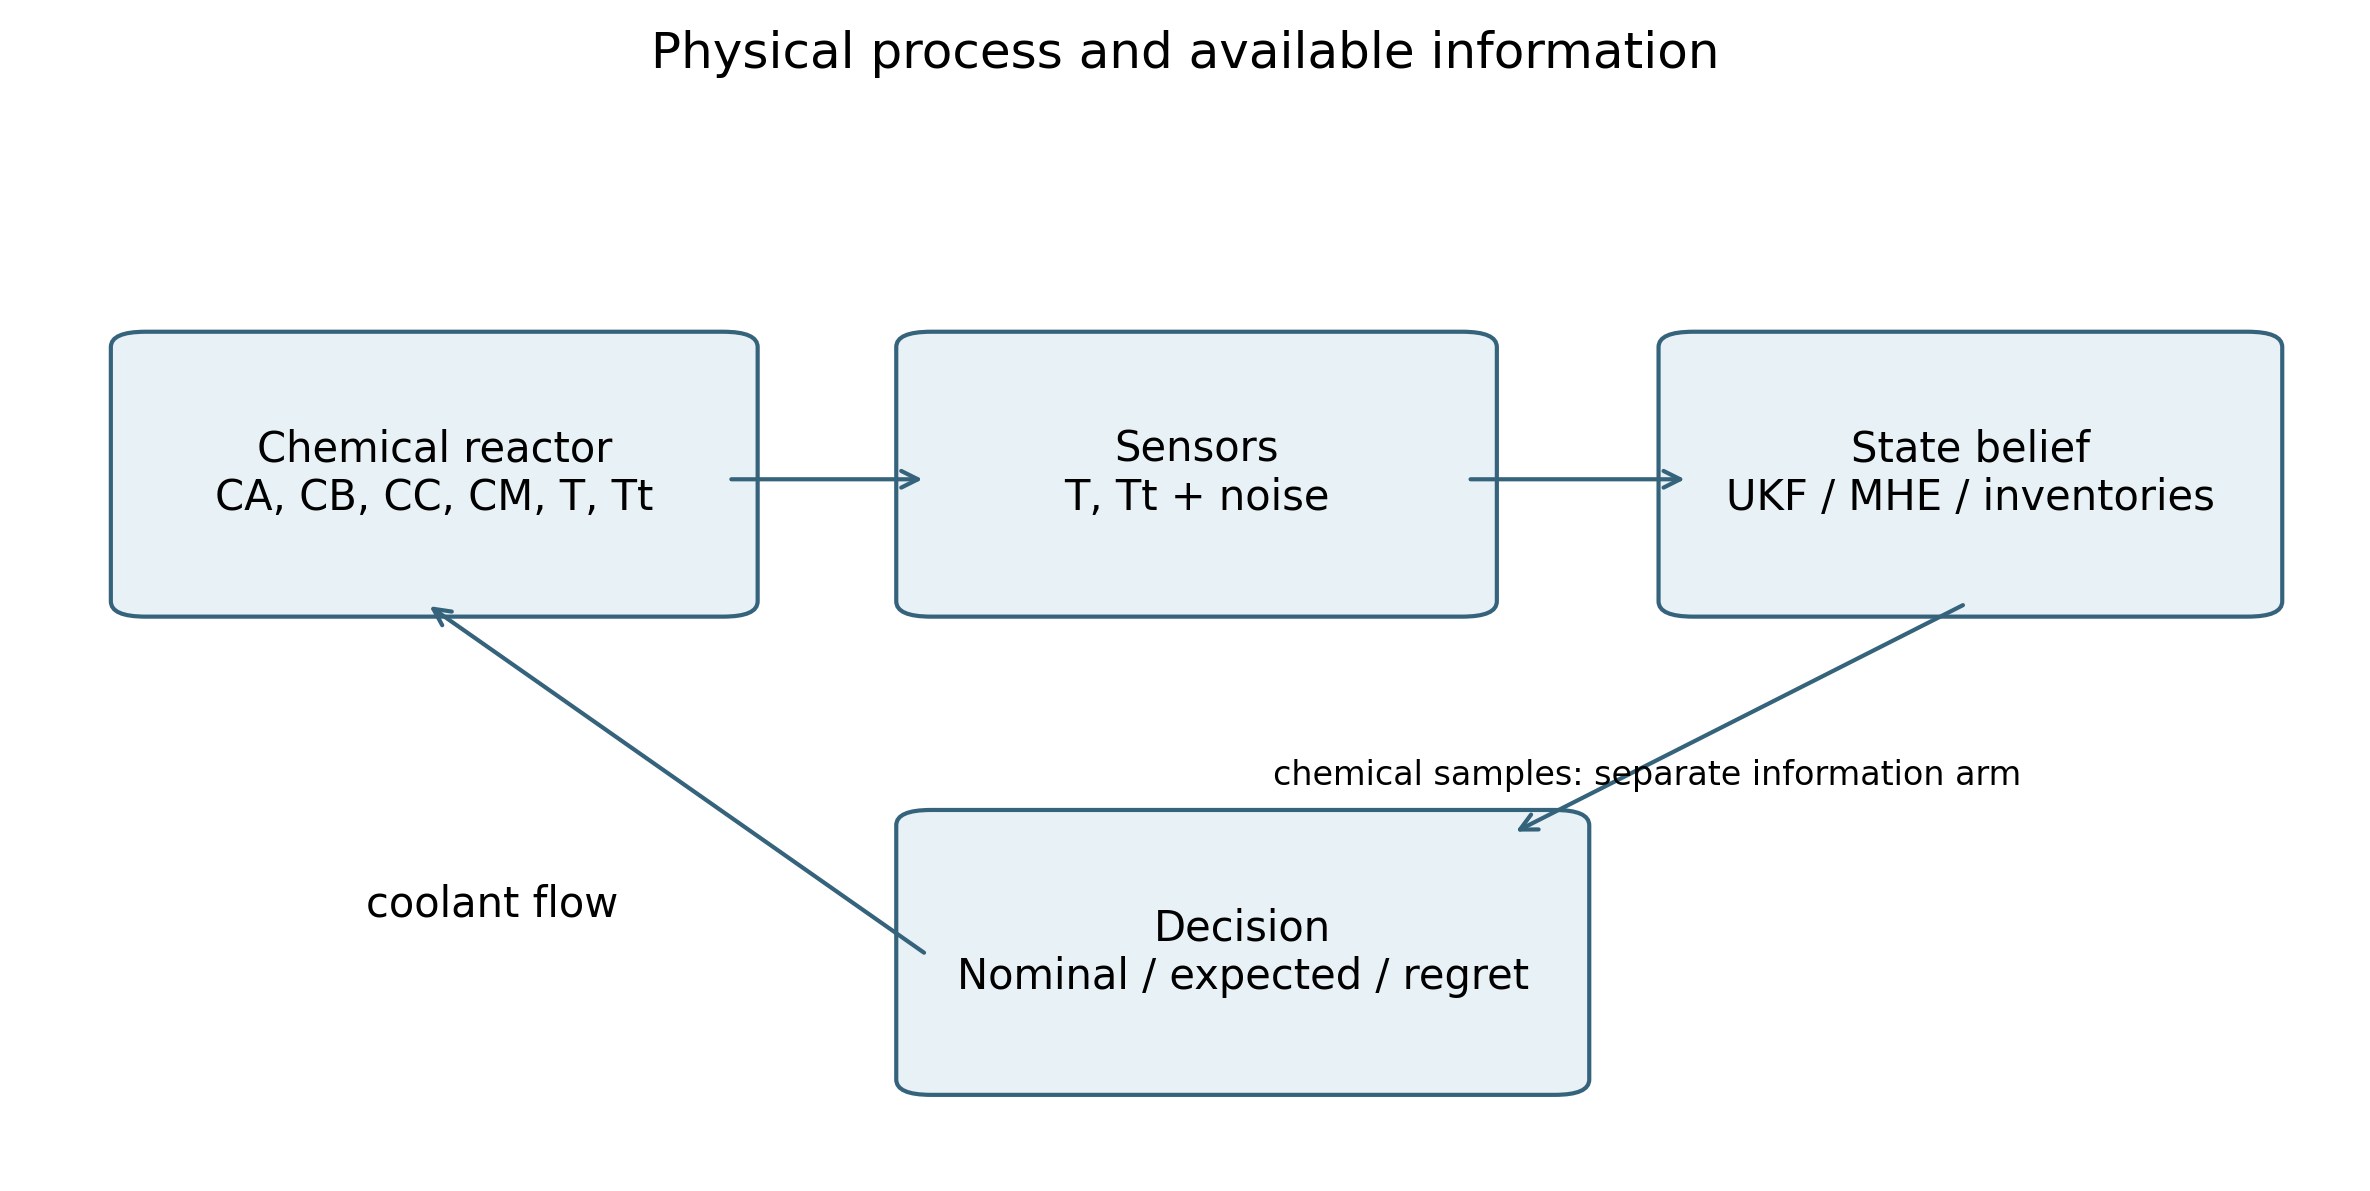
\includegraphics{figures/Figure_01.png}
\caption{Figure 1. Physical process and available information}
\end{figure}

\begin{figure}
\centering
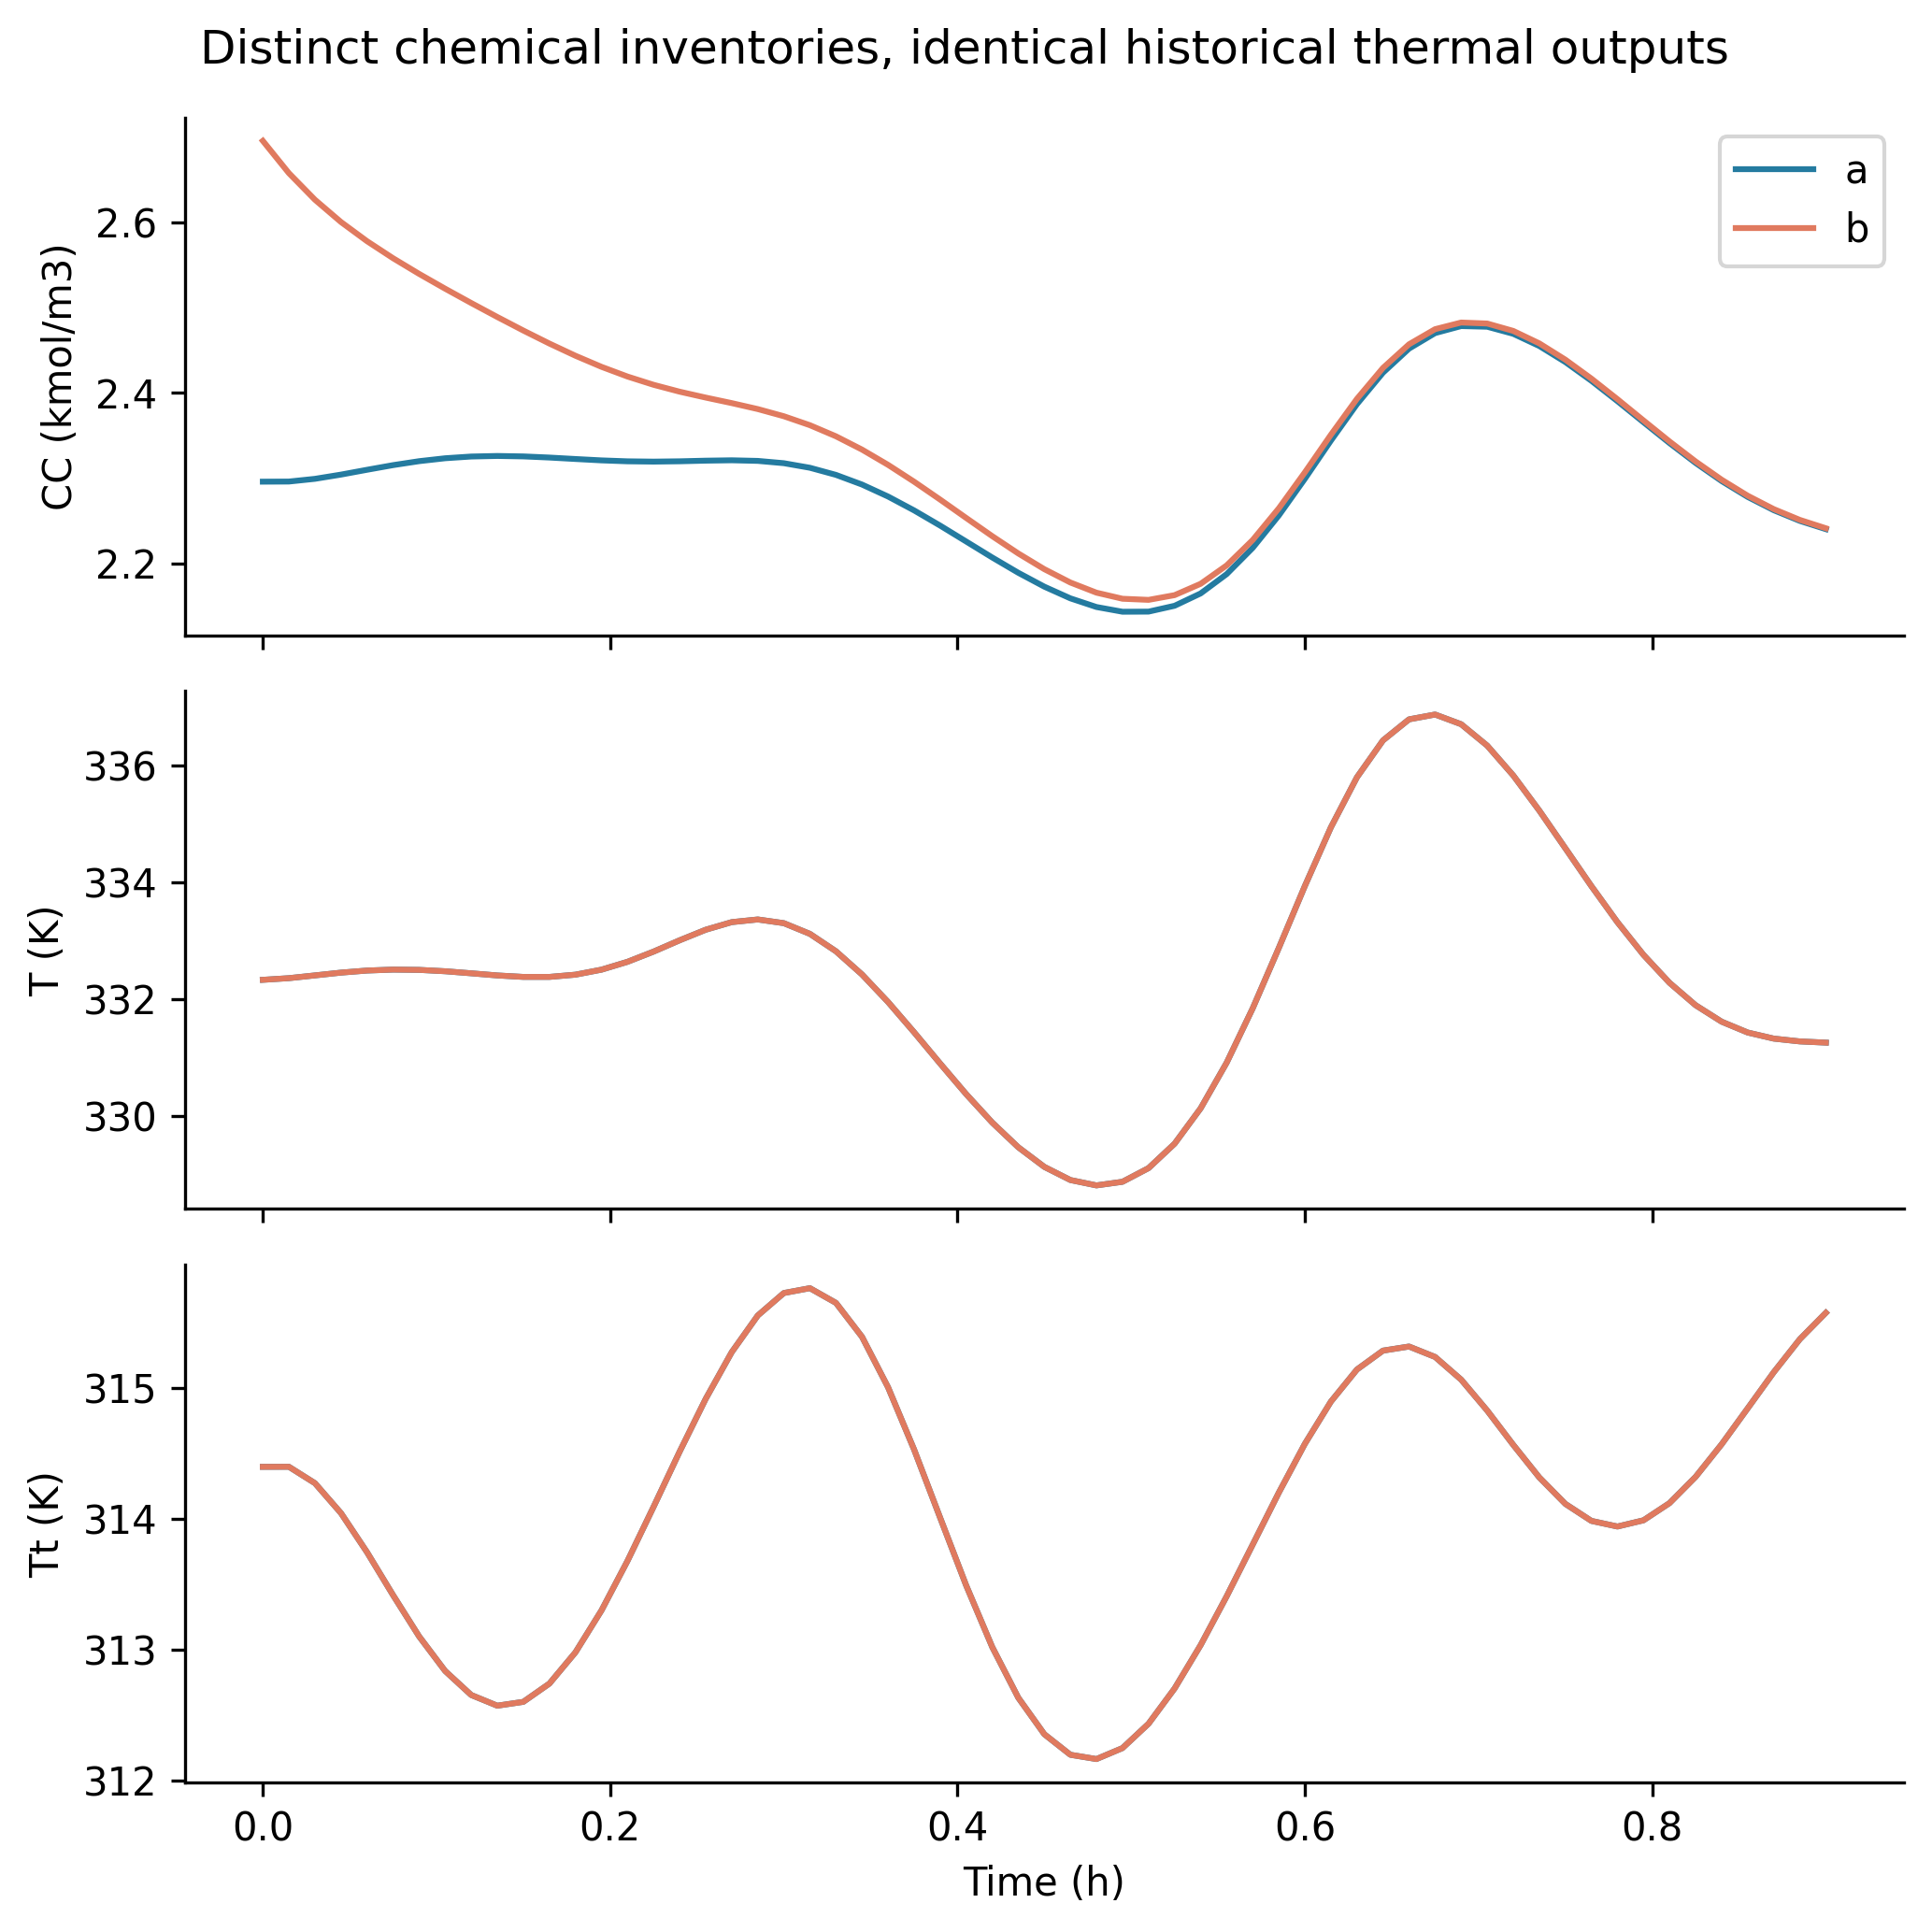
\includegraphics{figures/Figure_02.png}
\caption{Figure 2. Distinct chemical inventories, identical historical
thermal outputs}
\end{figure}

\begin{figure}
\centering
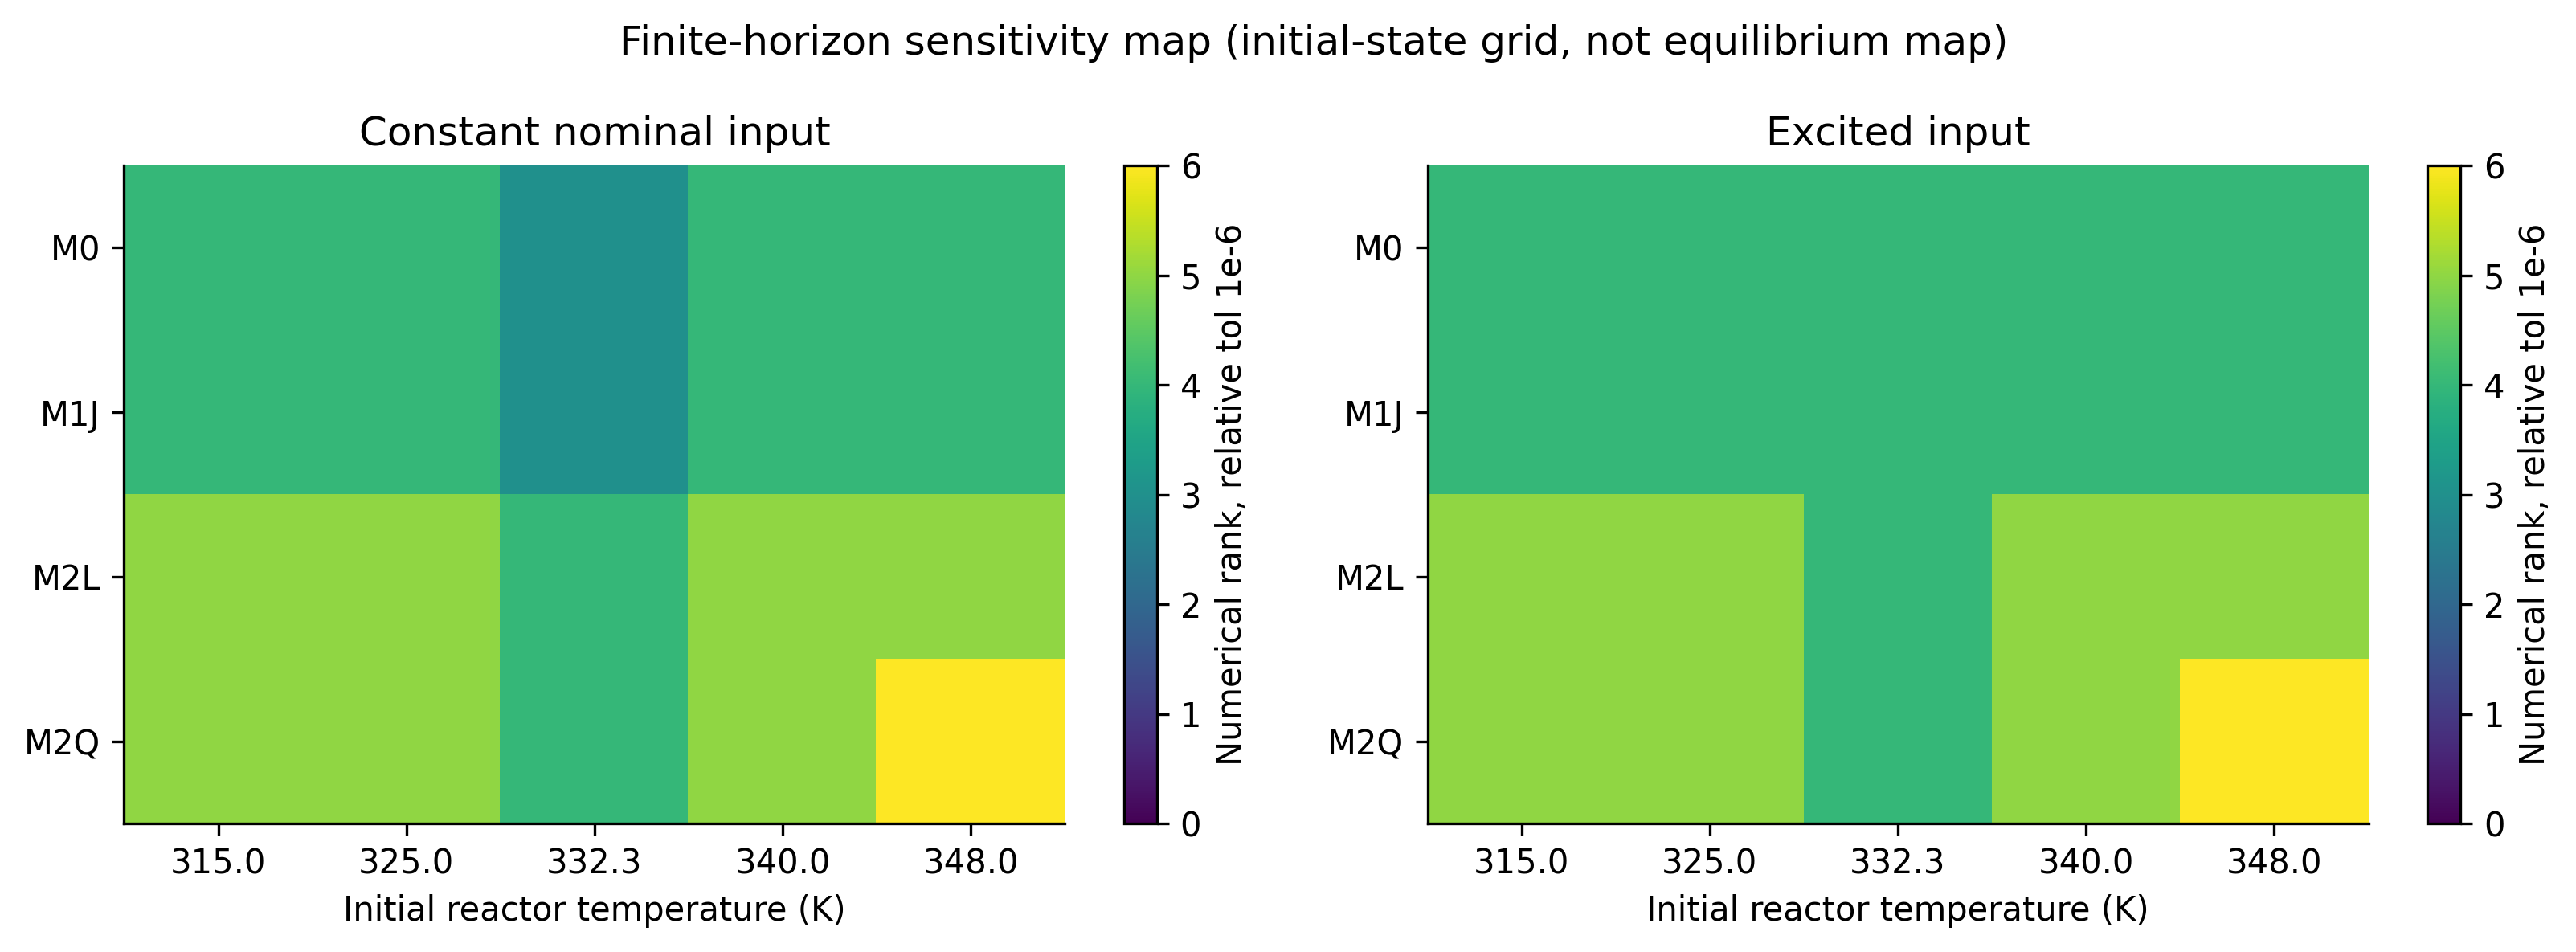
\includegraphics{figures/Figure_03.png}
\caption{Figure 3. Finite-horizon sensitivity map (initial-state grid,
not equilibrium map)}
\end{figure}

\begin{figure}
\centering
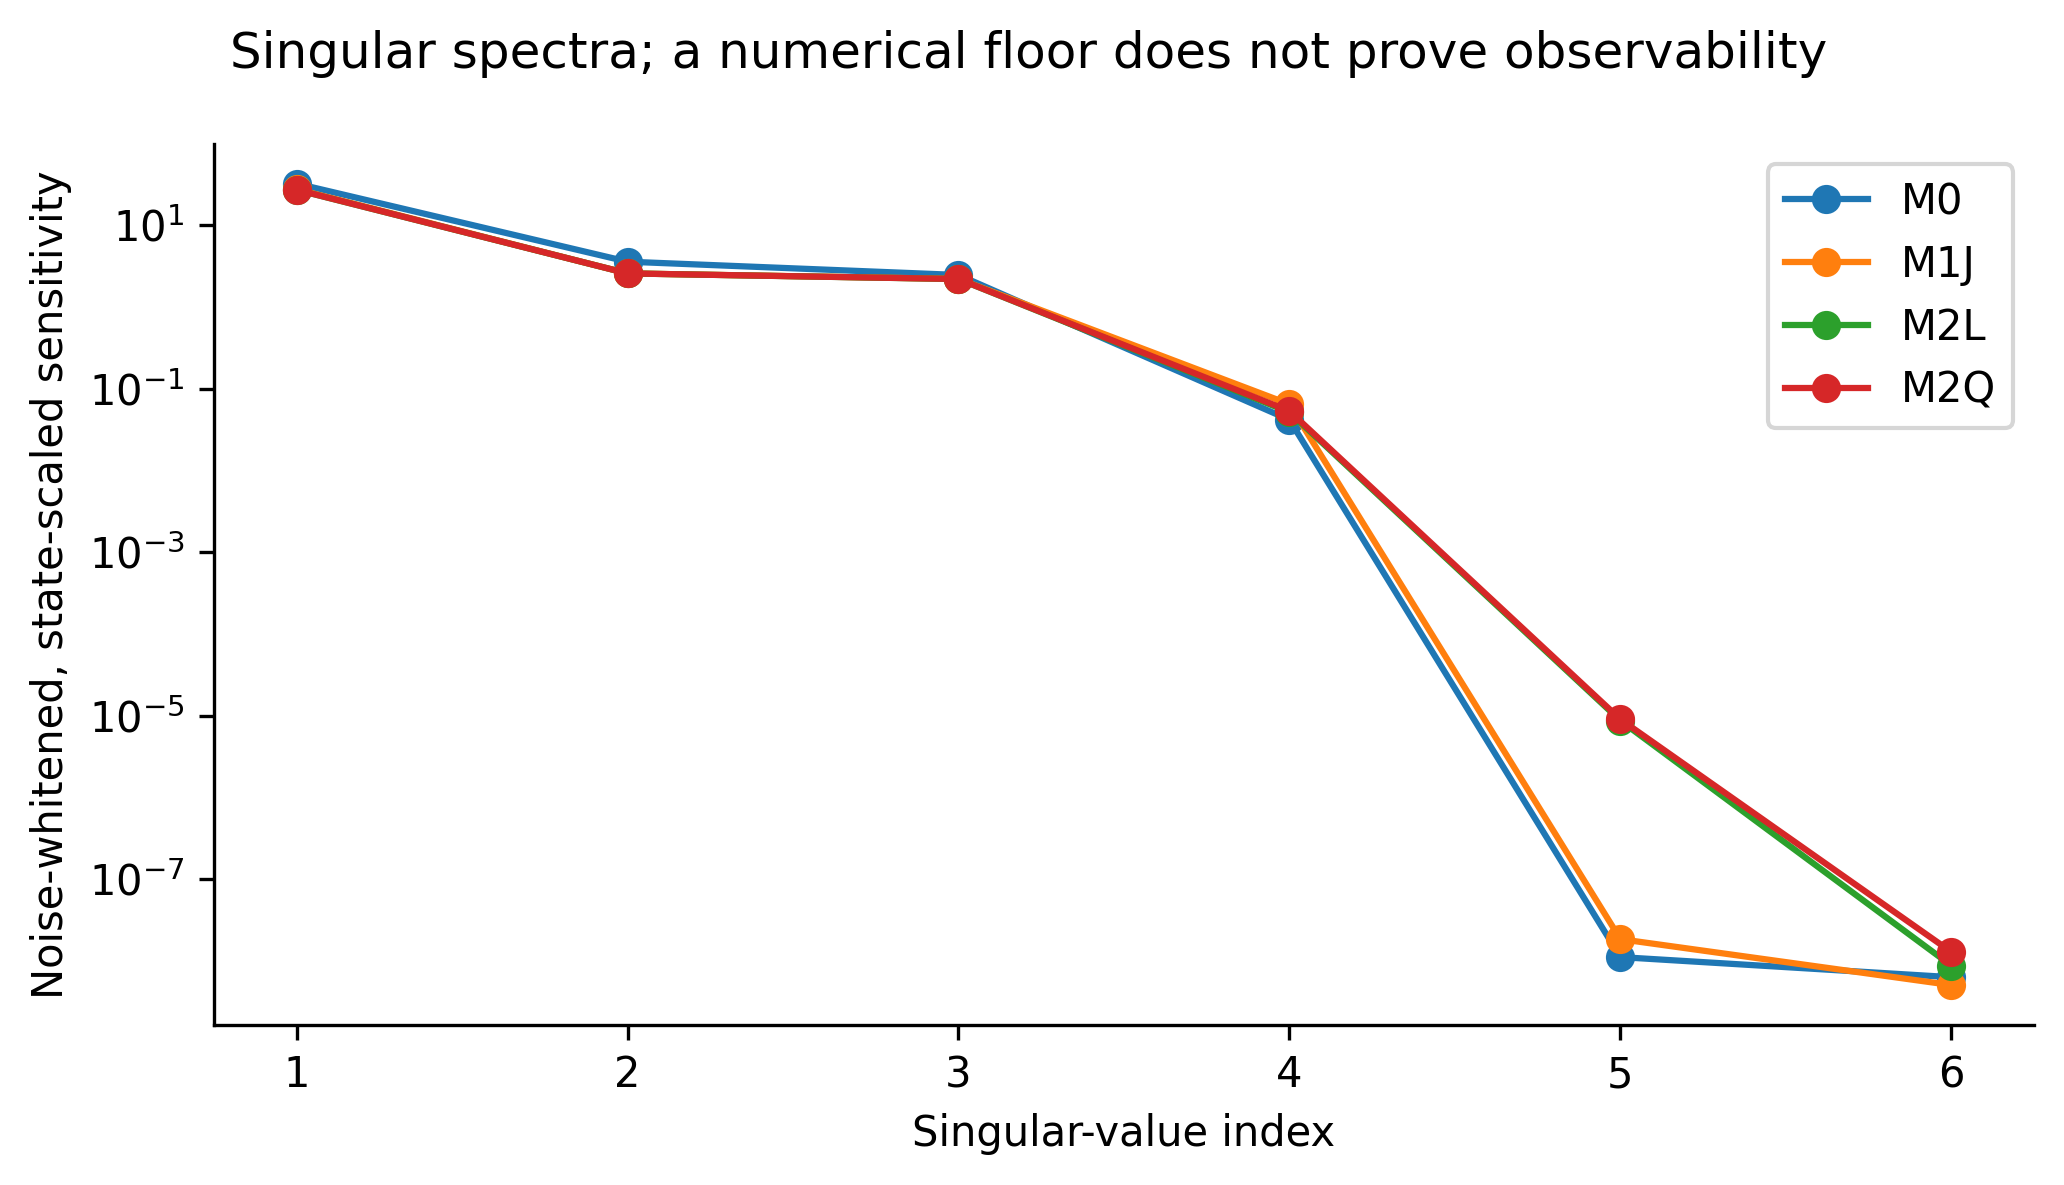
\includegraphics{figures/Figure_04.png}
\caption{Figure 4. Singular spectra; a numerical floor does not prove
observability}
\end{figure}

\begin{figure}
\centering
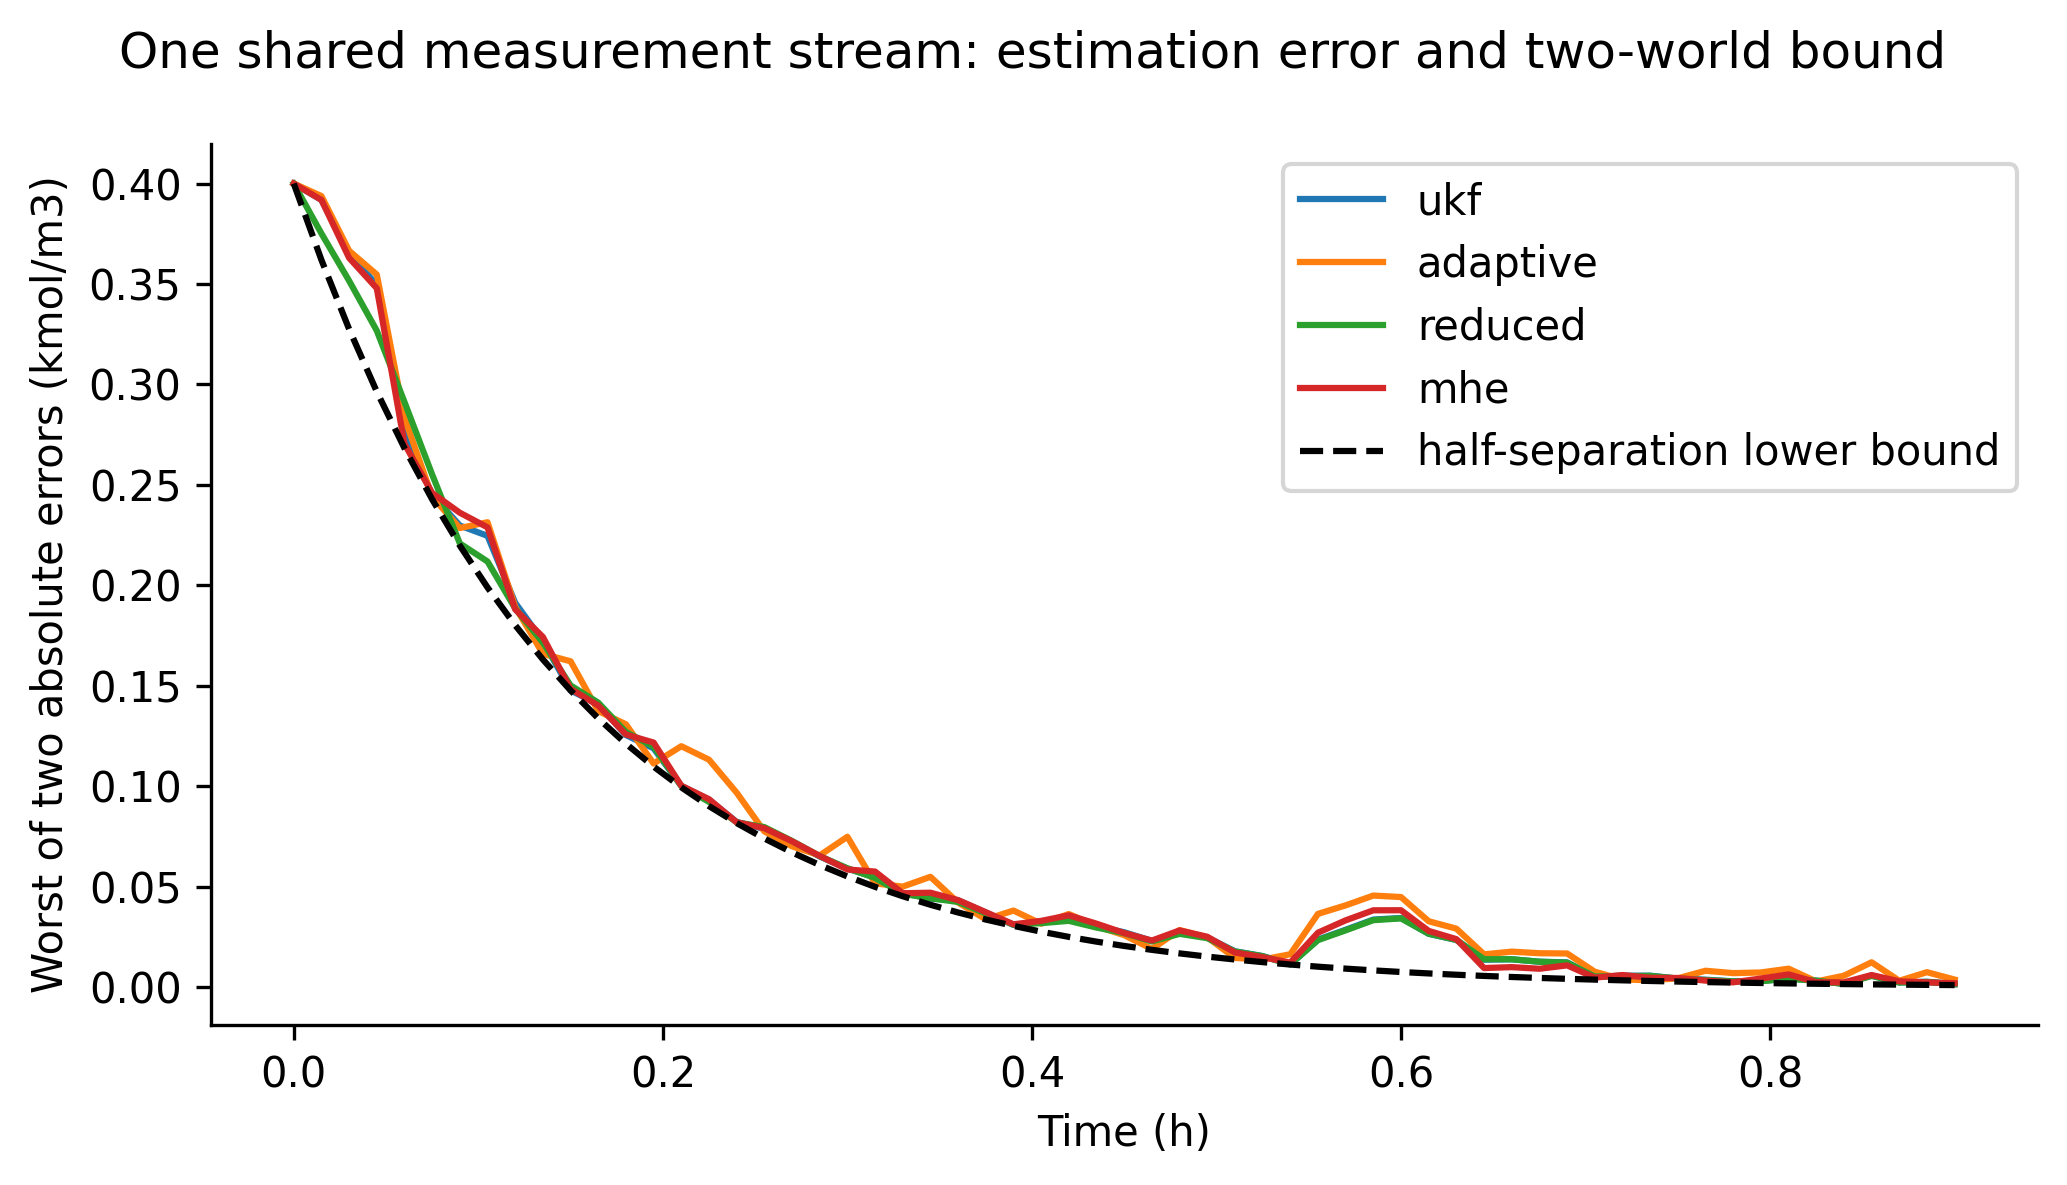
\includegraphics{figures/Figure_05.png}
\caption{Figure 5. One shared measurement stream: estimation error and
two-world bound}
\end{figure}

\begin{figure}
\centering
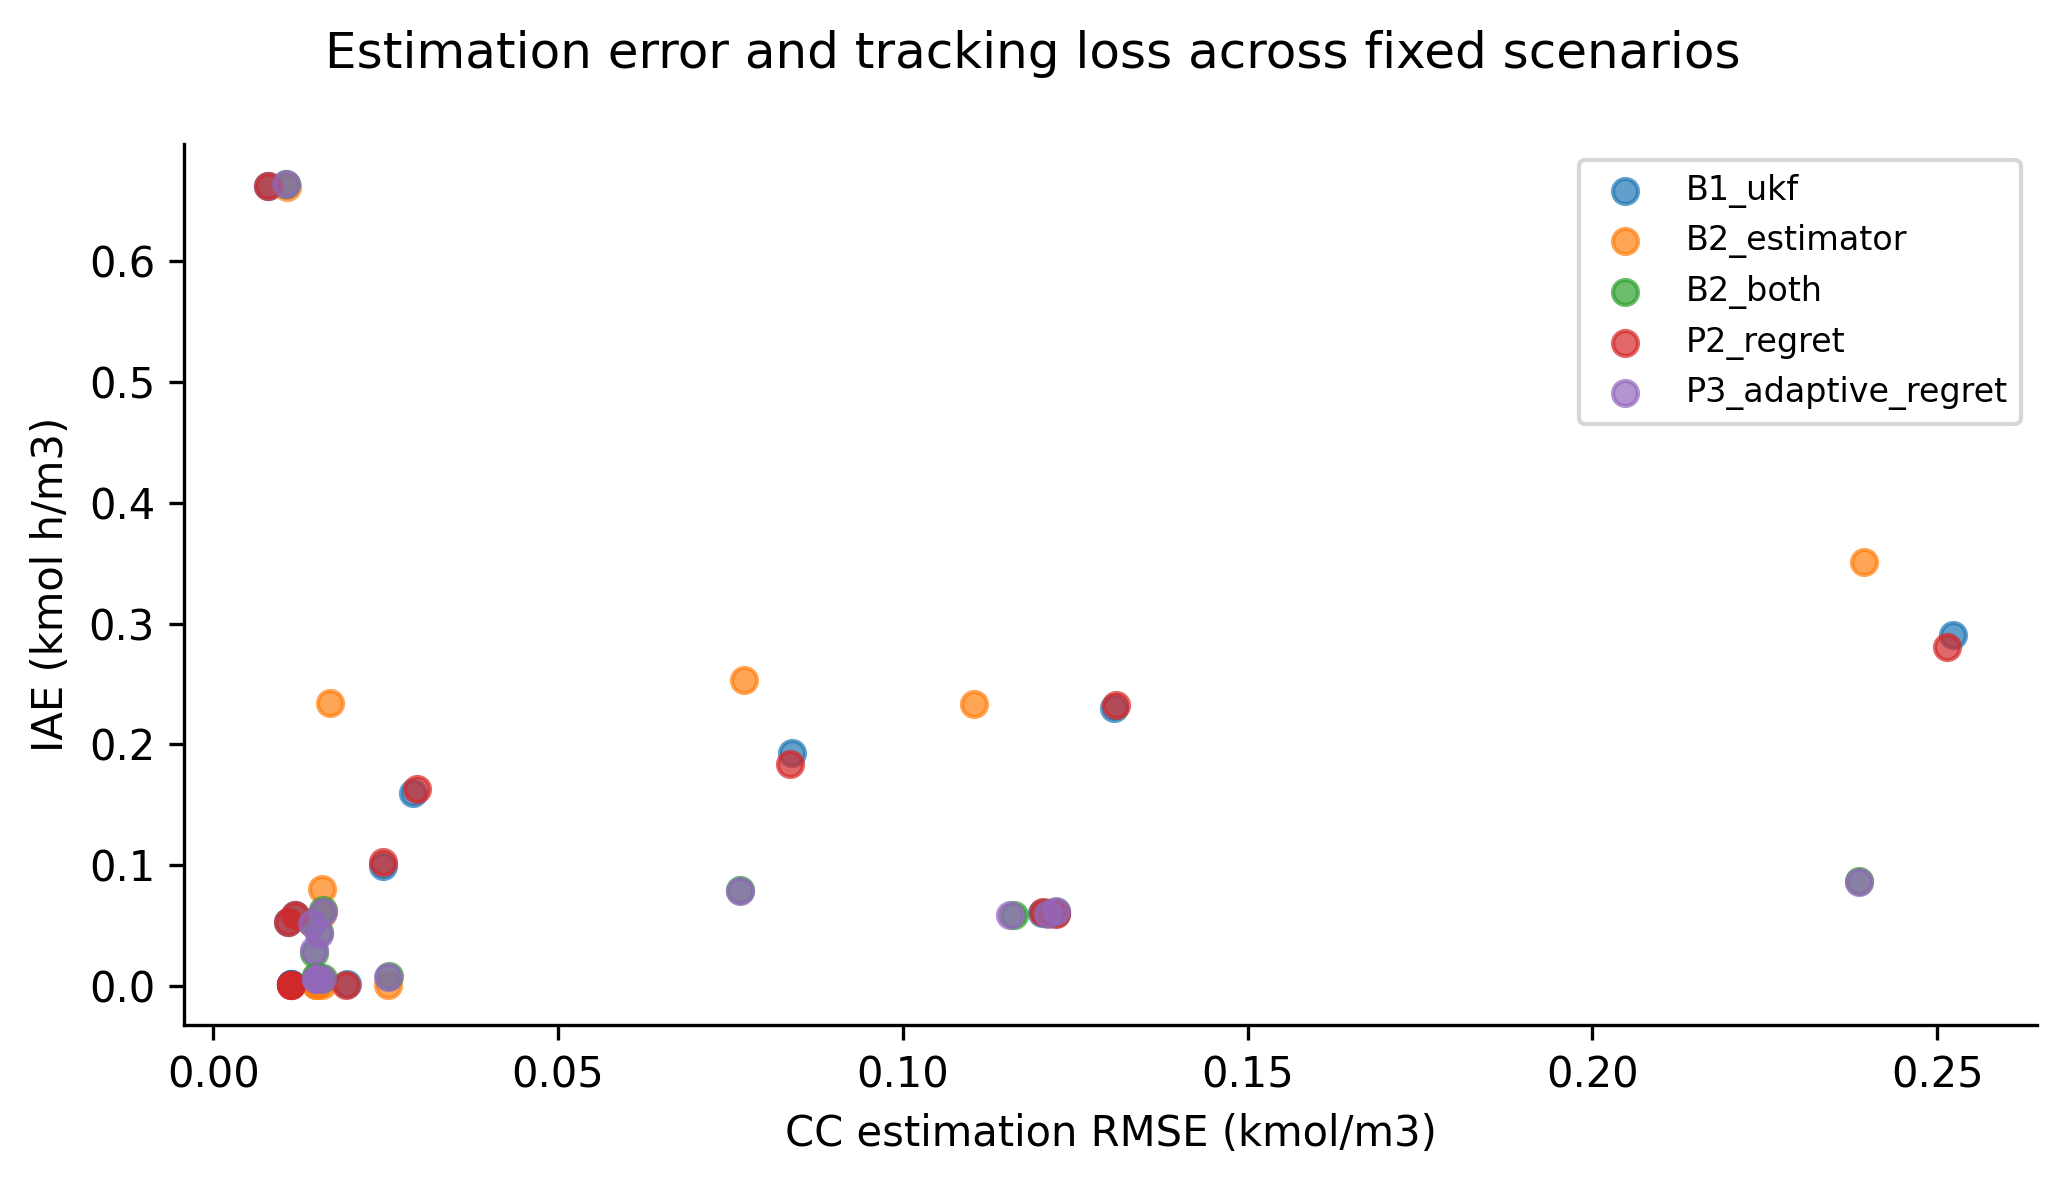
\includegraphics{figures/Figure_06.png}
\caption{Figure 6. Estimation error and tracking loss across fixed
scenarios}
\end{figure}

\begin{figure}
\centering
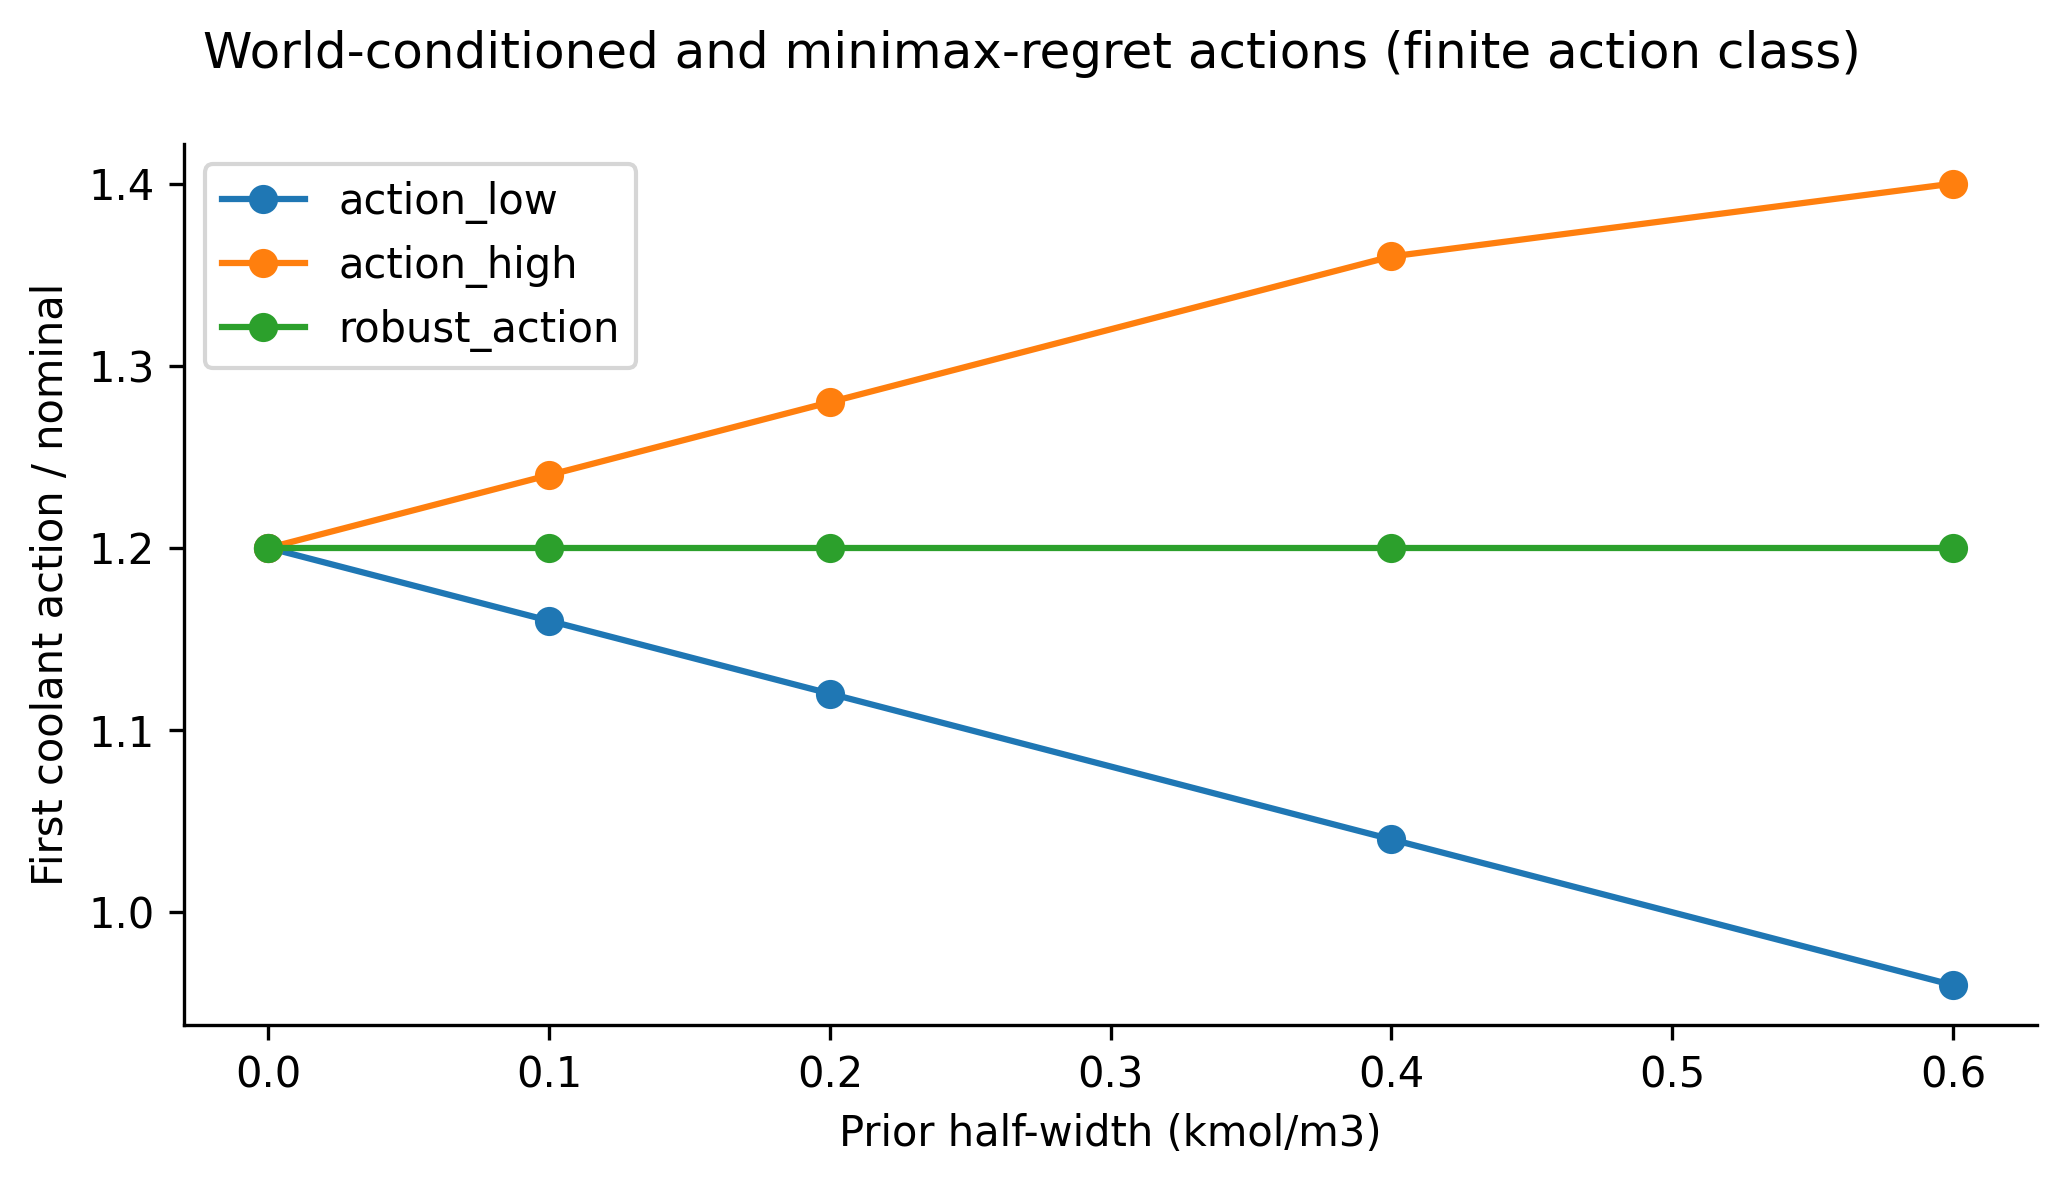
\includegraphics{figures/Figure_07.png}
\caption{Figure 7. World-conditioned and minimax-regret actions (finite
action class)}
\end{figure}

\begin{figure}
\centering
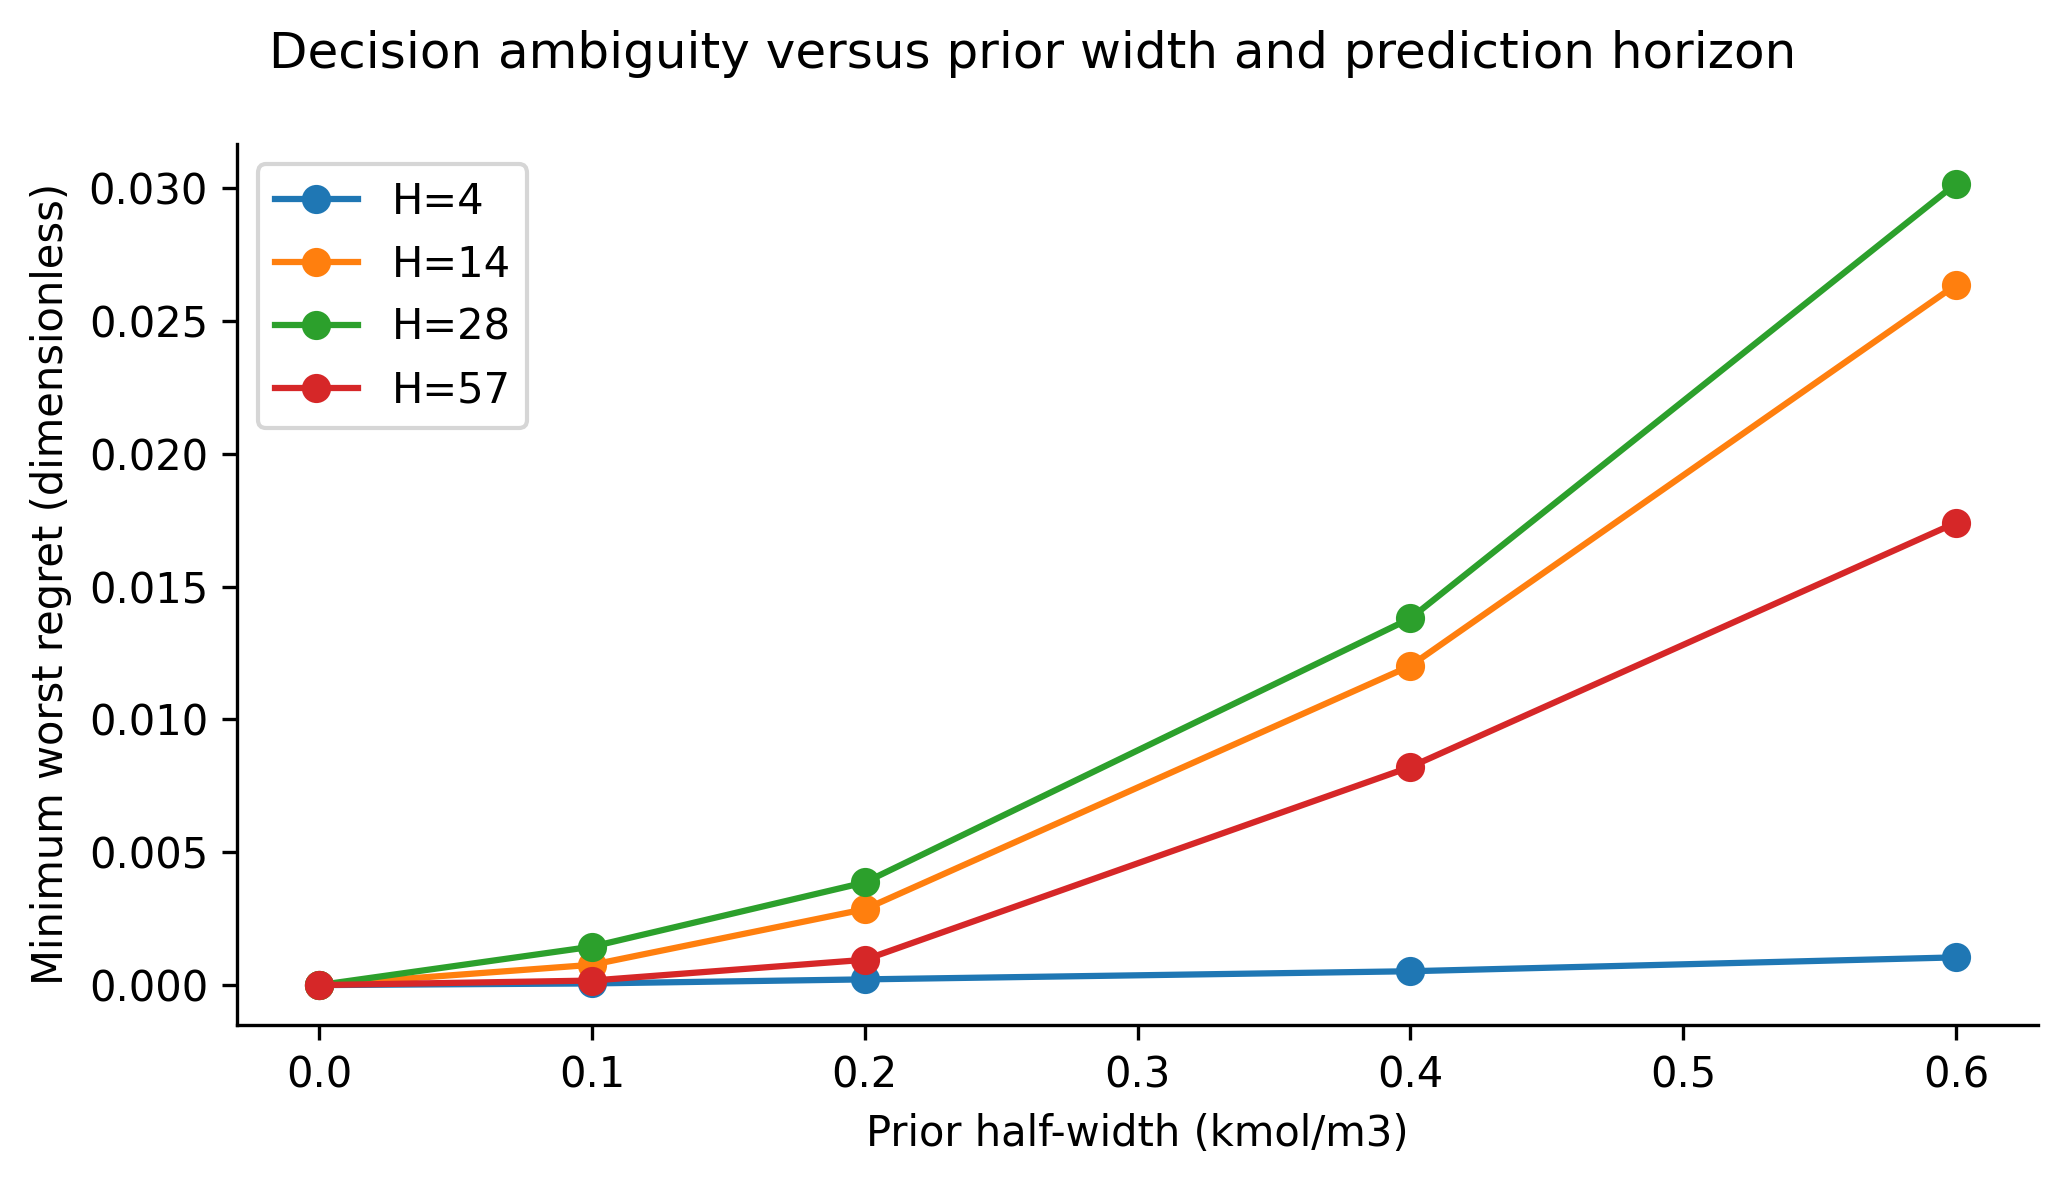
\includegraphics{figures/Figure_08.png}
\caption{Figure 8. Decision ambiguity versus prior width and prediction
horizon}
\end{figure}

\begin{figure}
\centering
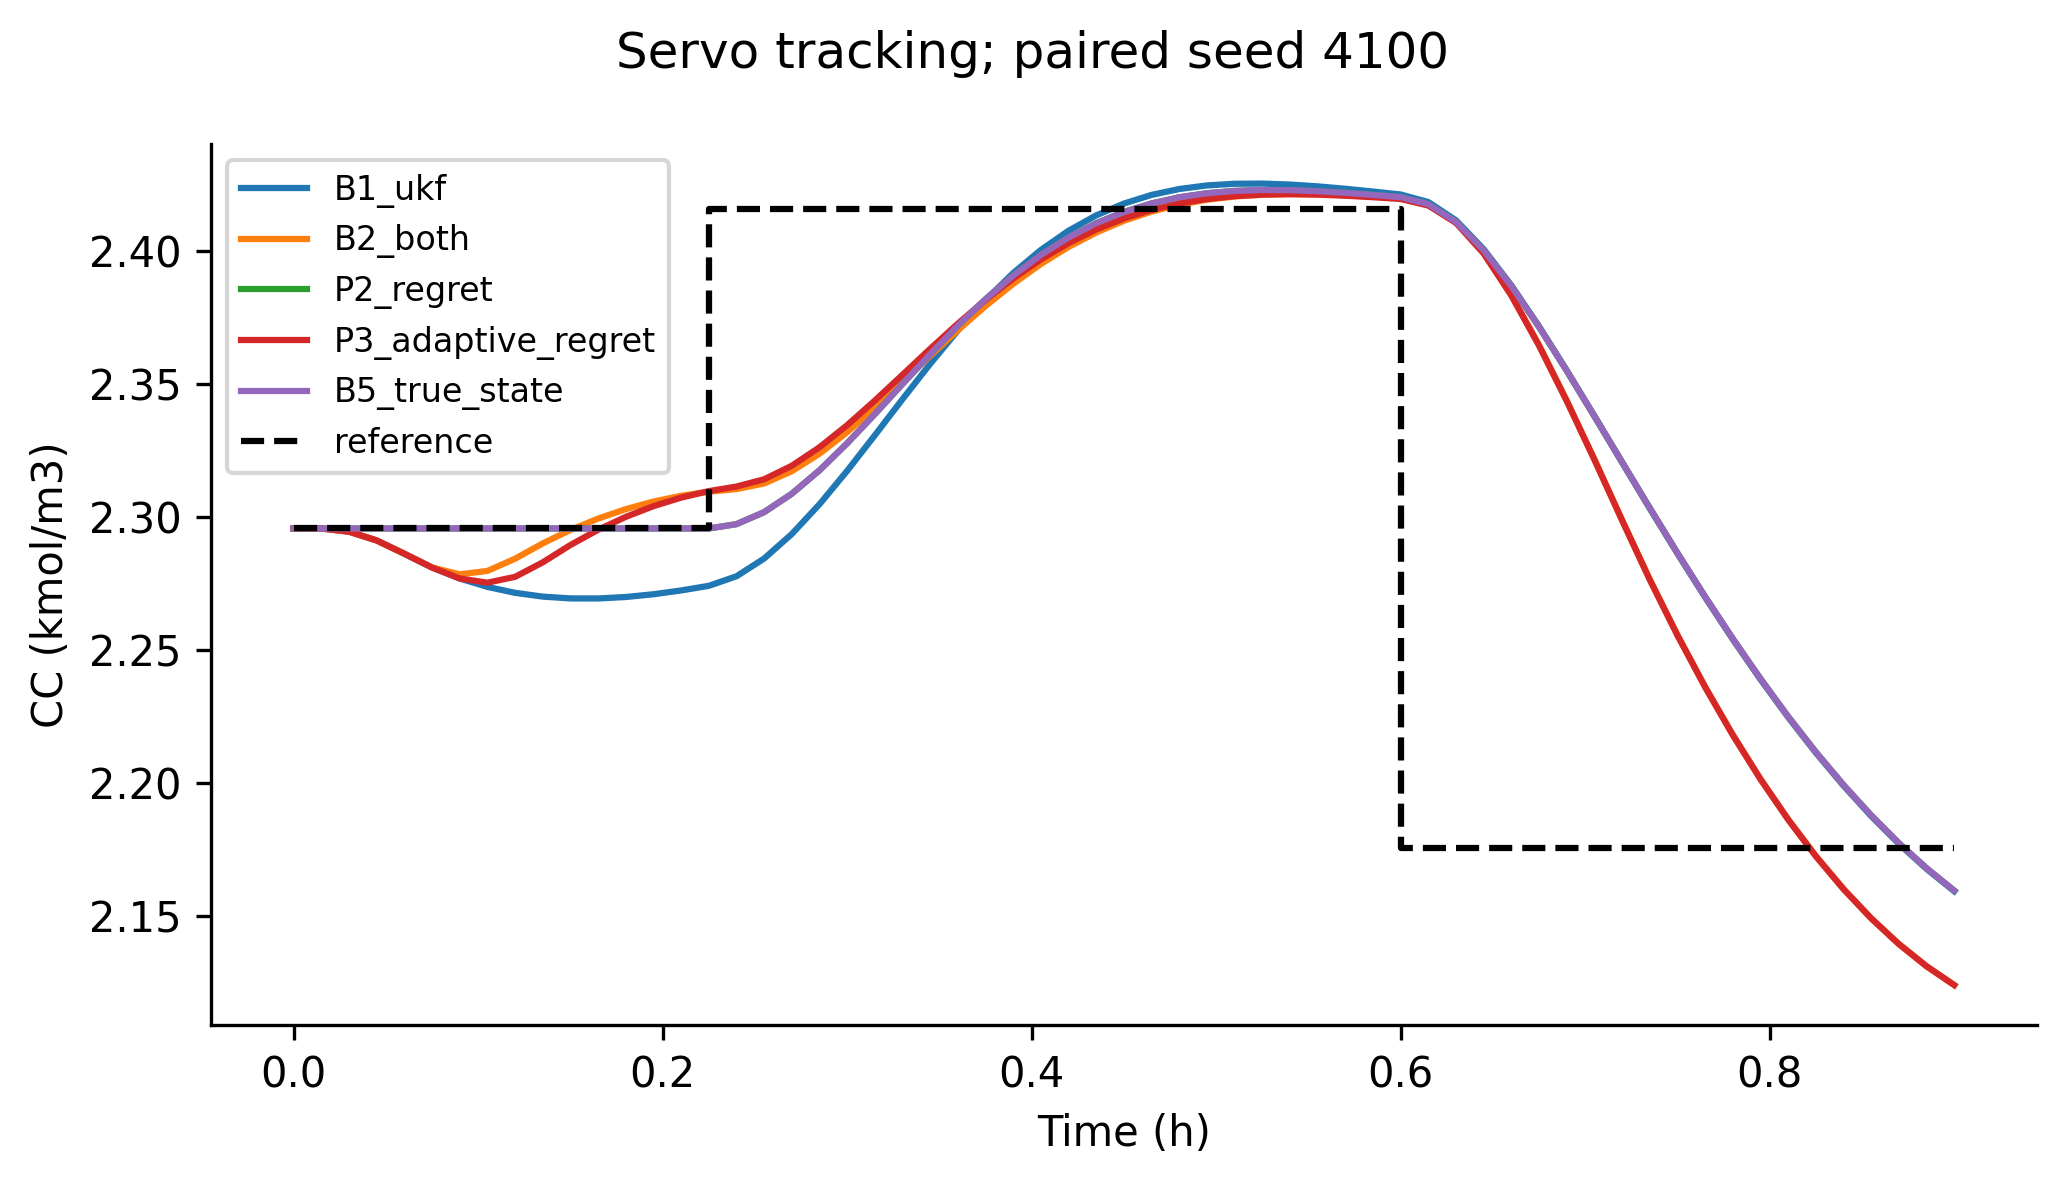
\includegraphics{figures/Figure_09.png}
\caption{Figure 9. Servo tracking; paired seed 4100}
\end{figure}

\begin{figure}
\centering
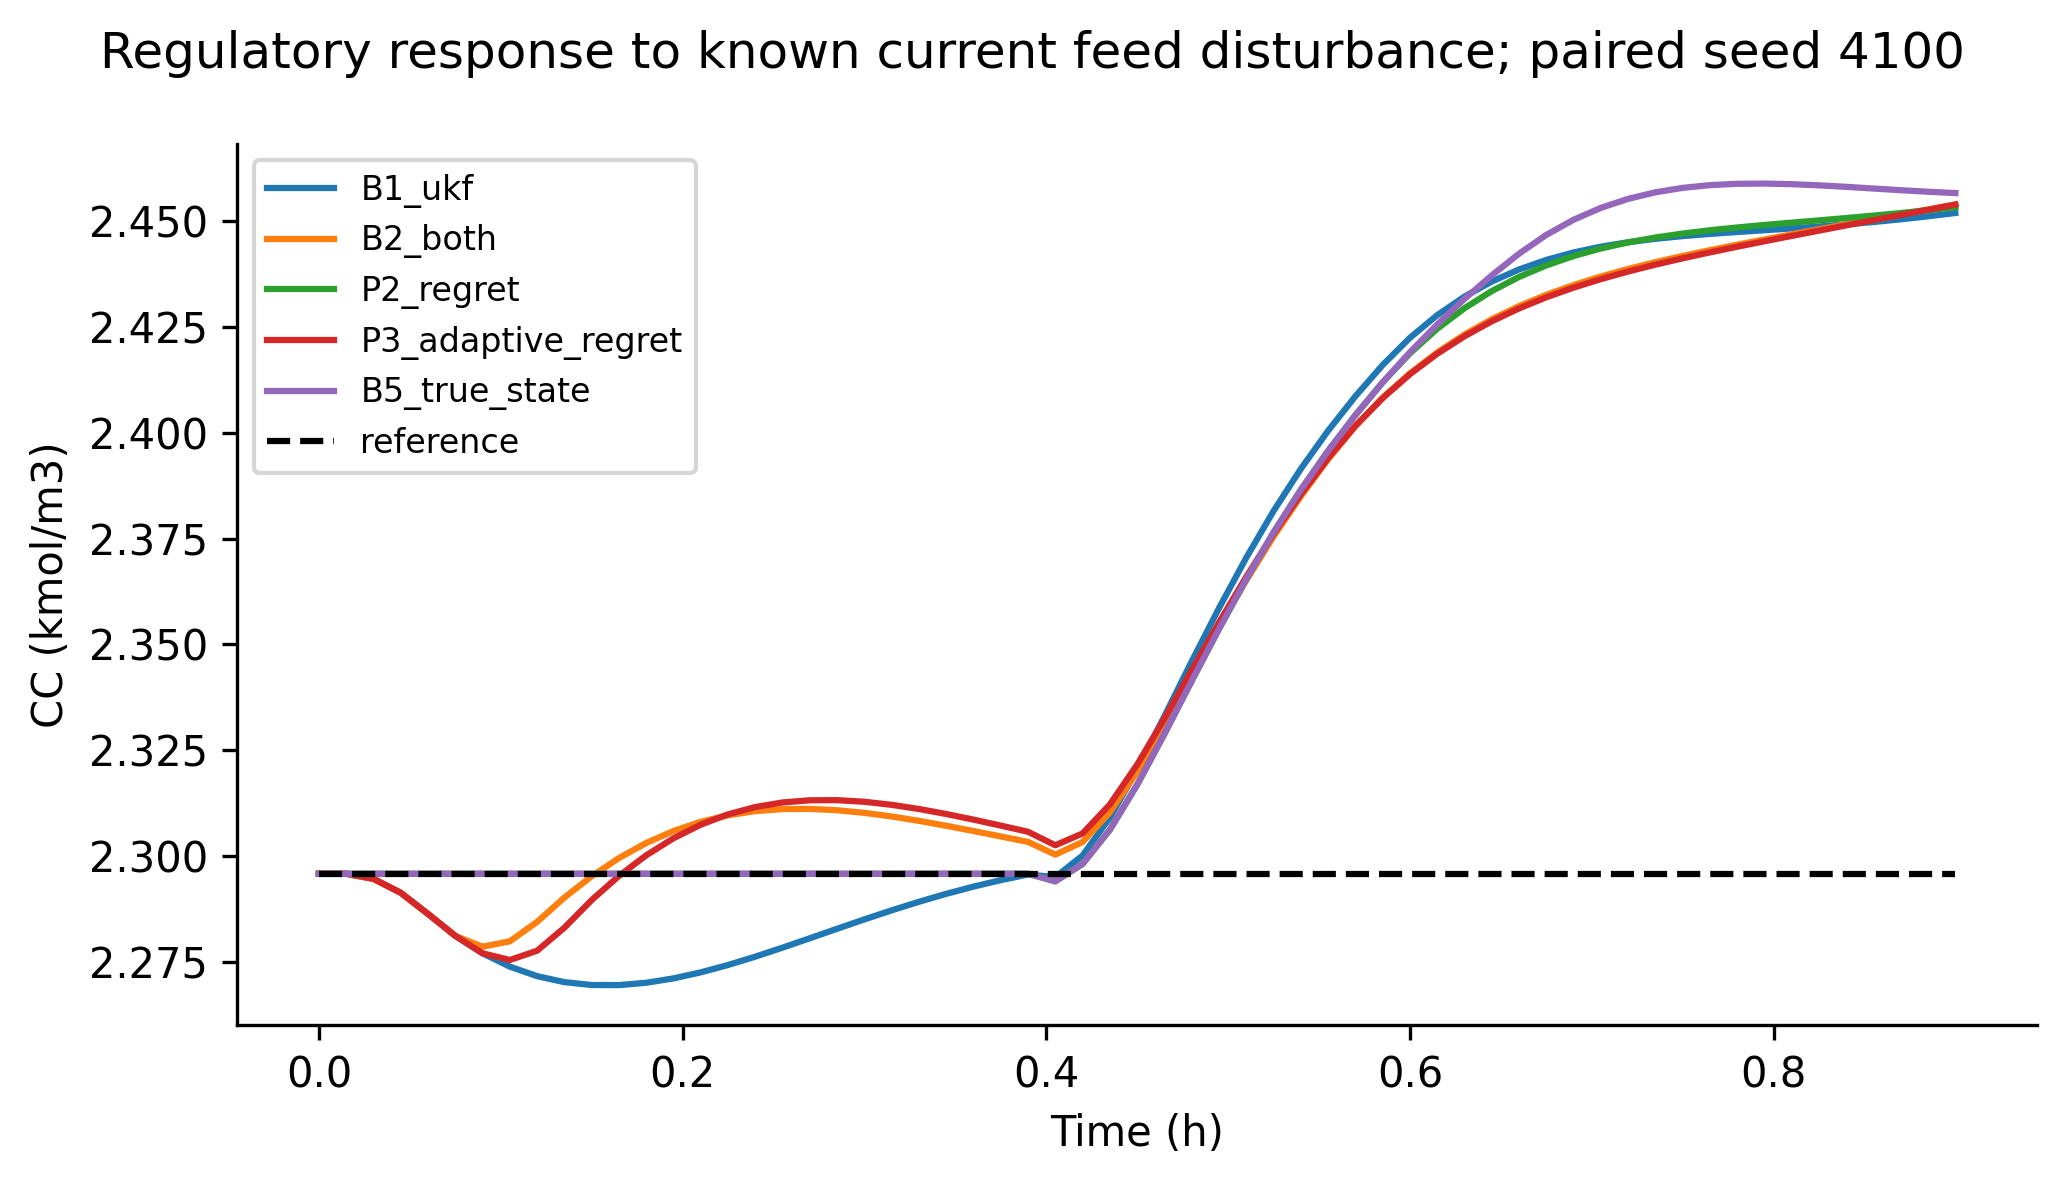
\includegraphics{figures/Figure_10.png}
\caption{Figure 10. Regulatory response to known current feed
disturbance; paired seed 4100}
\end{figure}

\begin{figure}
\centering
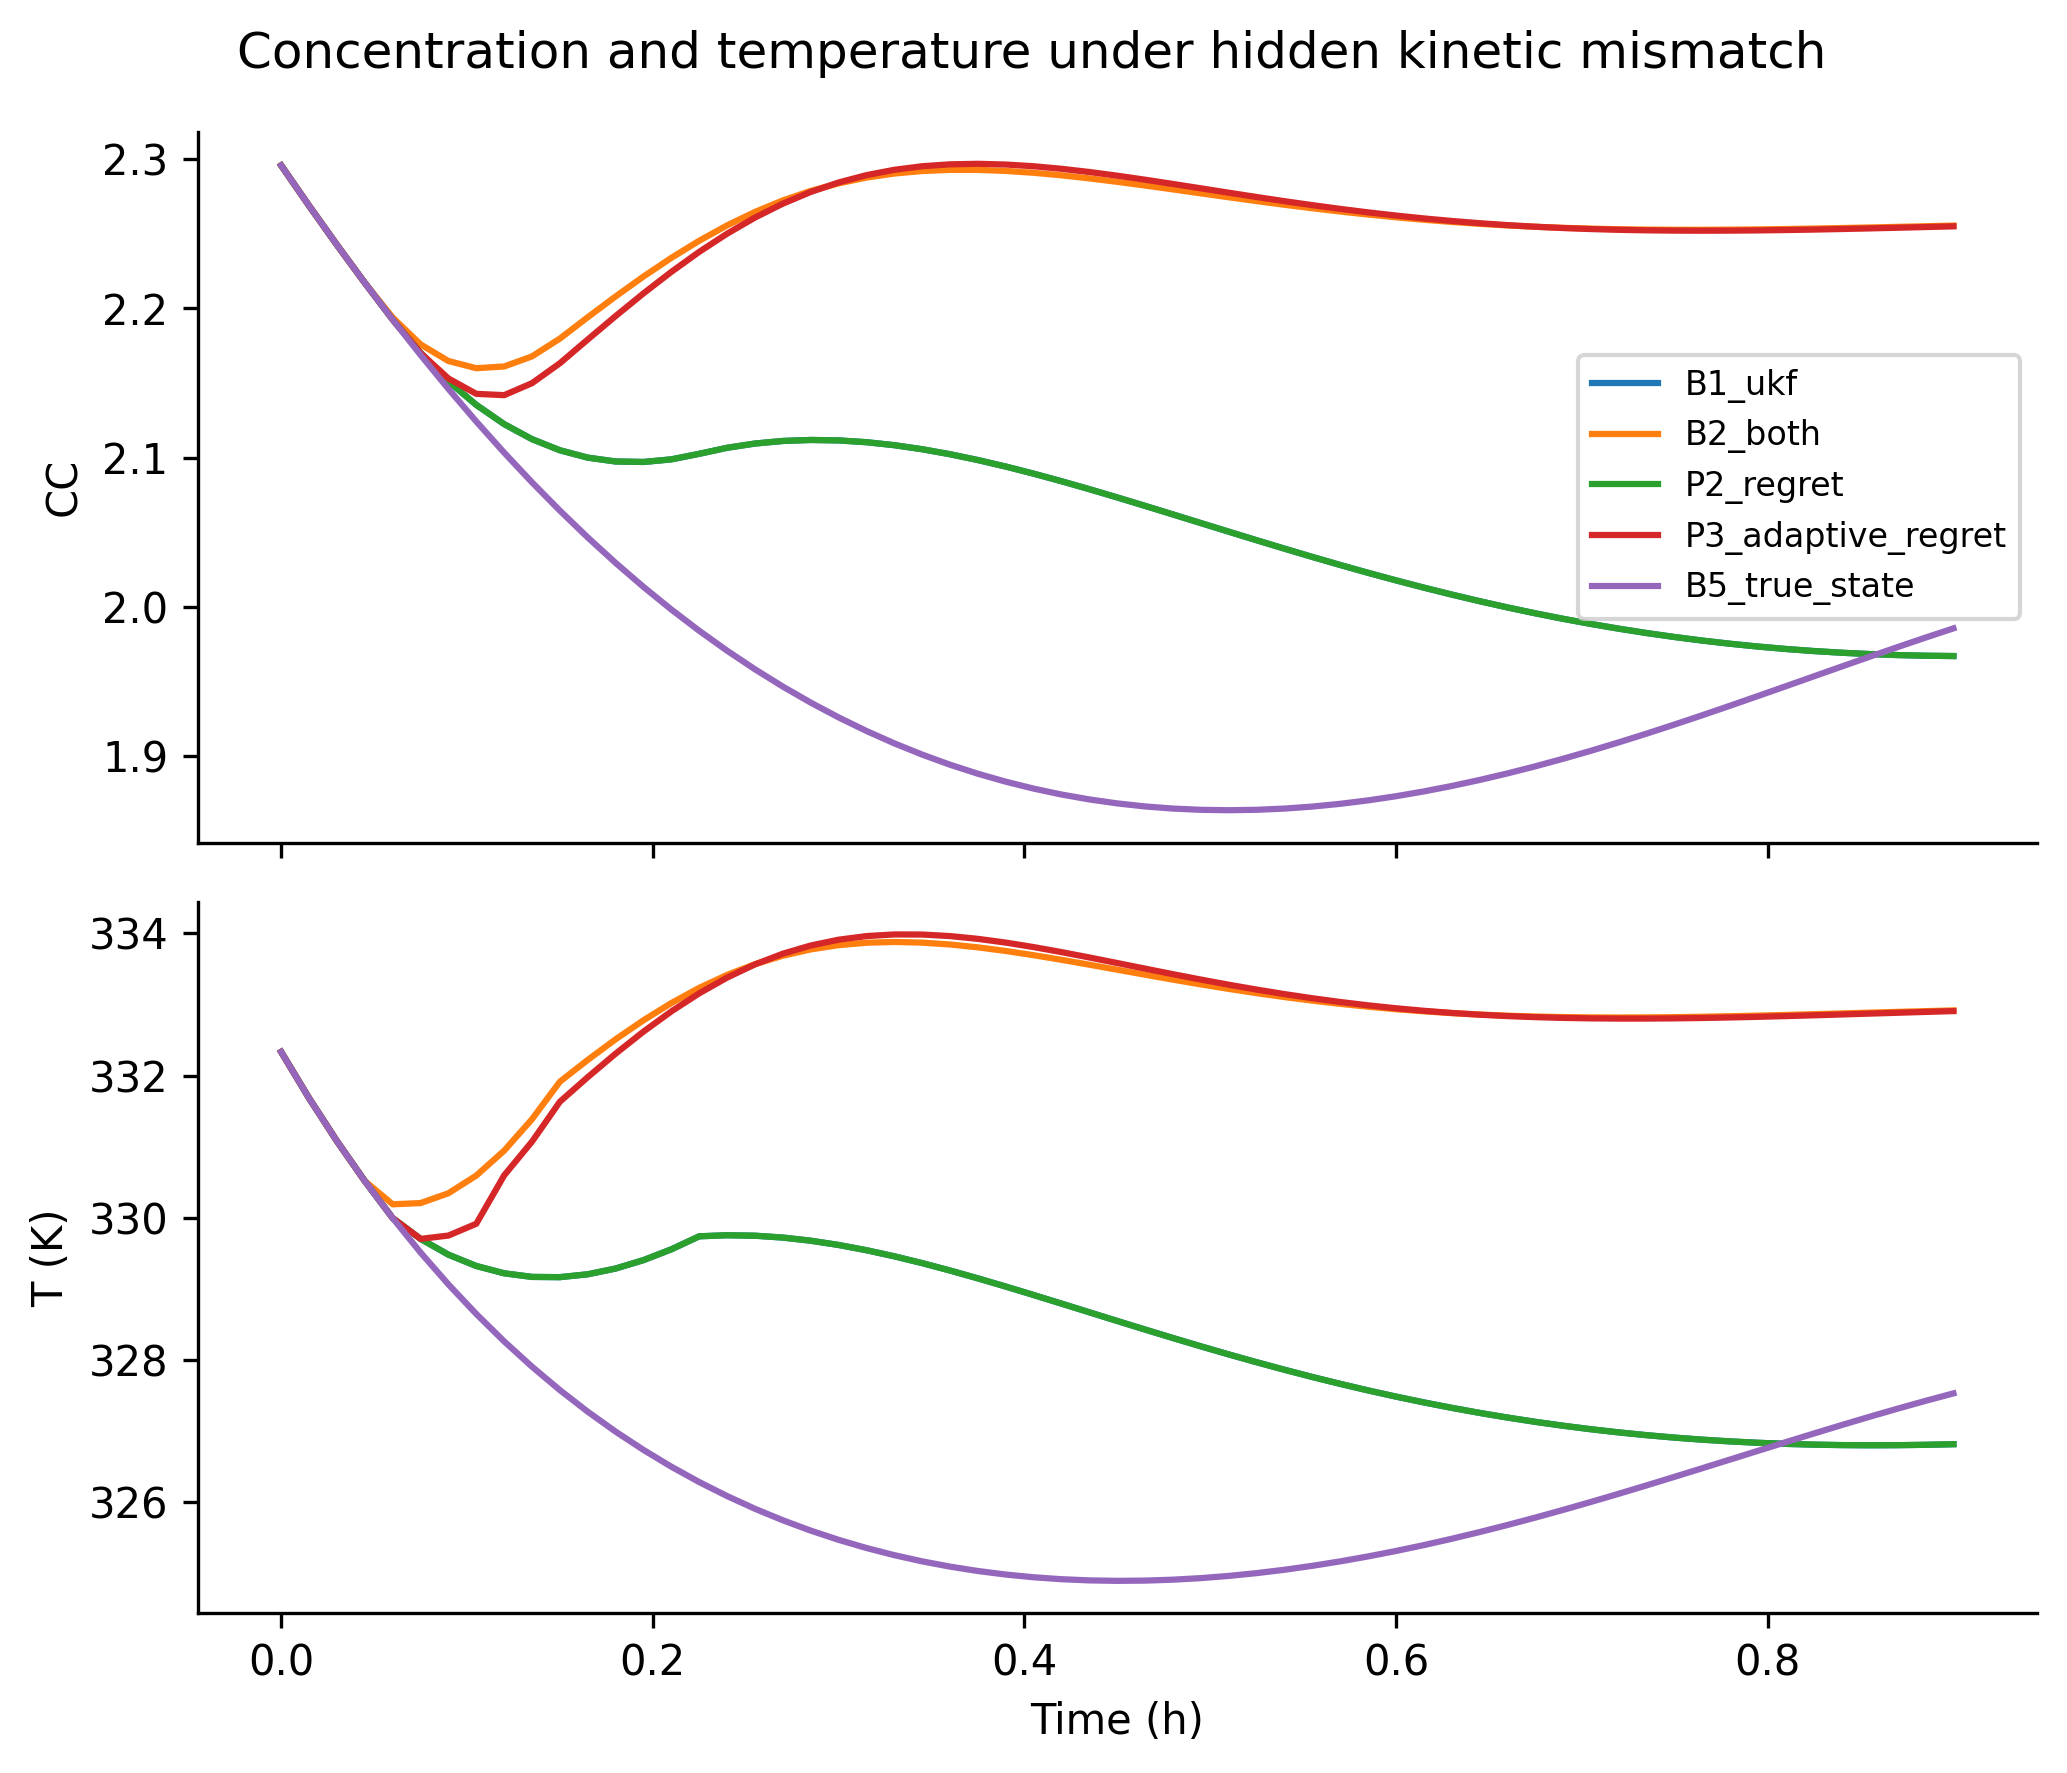
\includegraphics{figures/Figure_11.png}
\caption{Figure 11. Concentration and temperature under hidden kinetic
mismatch}
\end{figure}

\begin{figure}
\centering
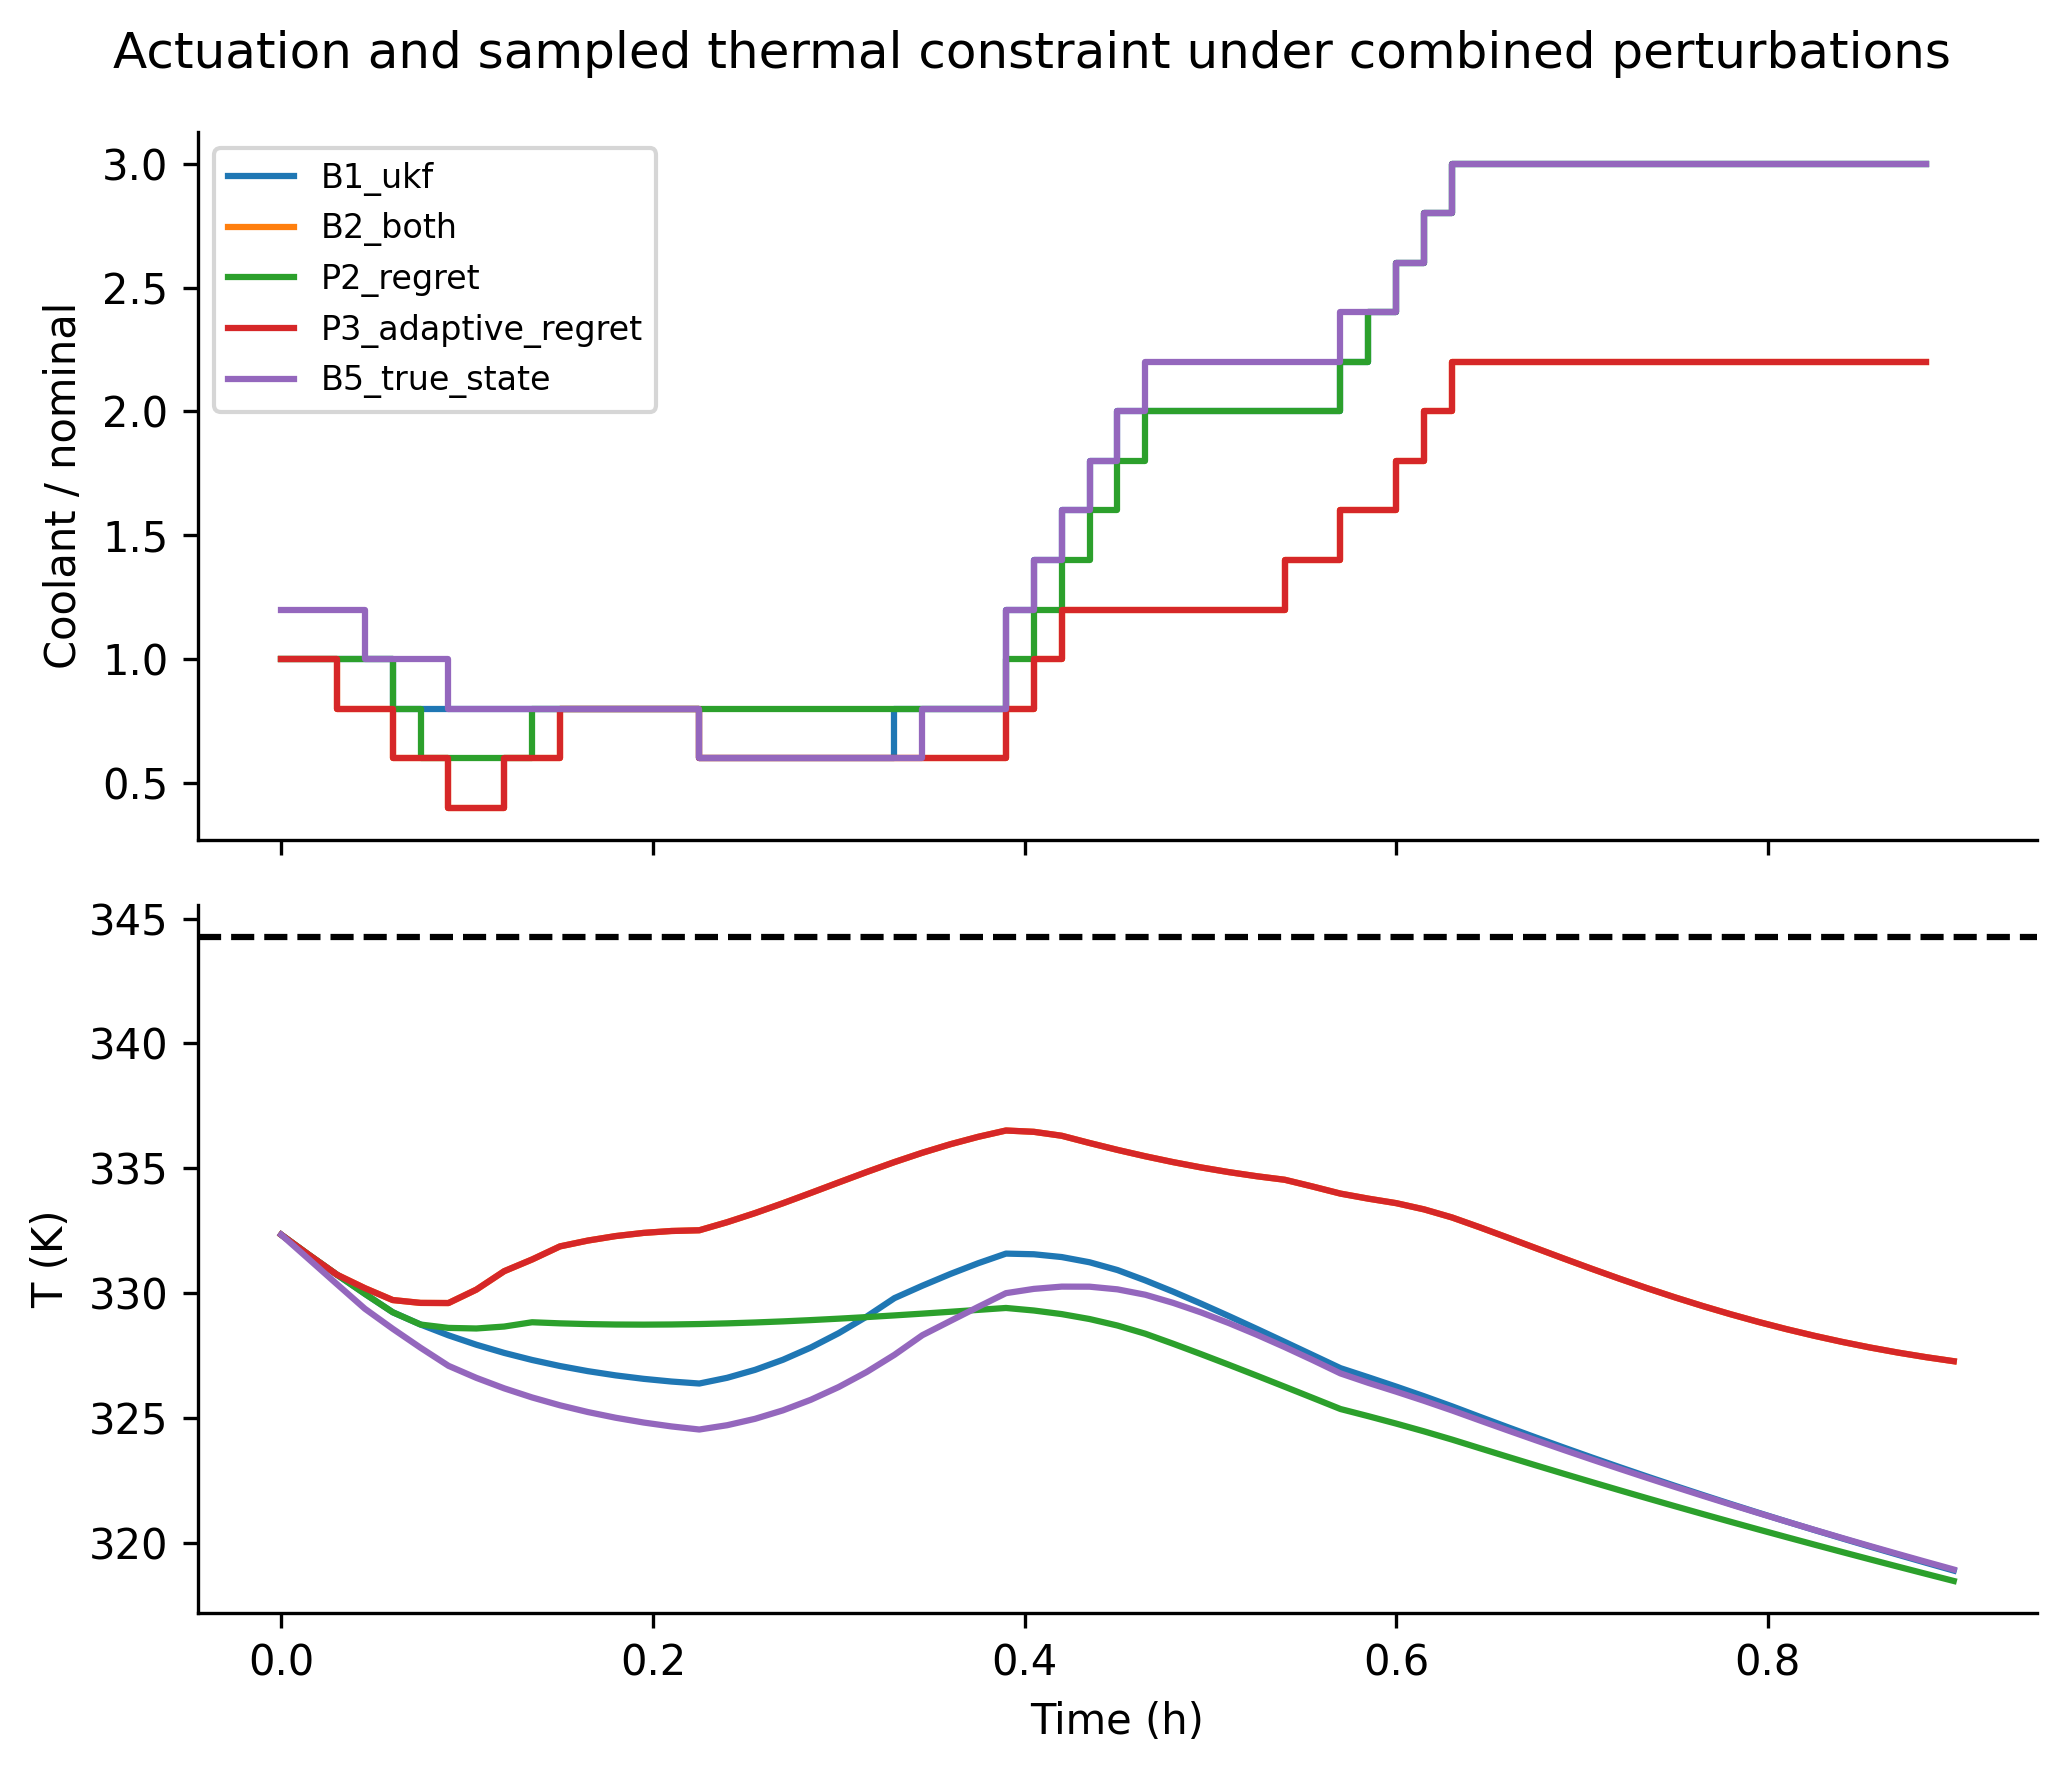
\includegraphics{figures/Figure_12.png}
\caption{Figure 12. Actuation and sampled thermal constraint under
combined perturbations}
\end{figure}

\begin{figure}
\centering
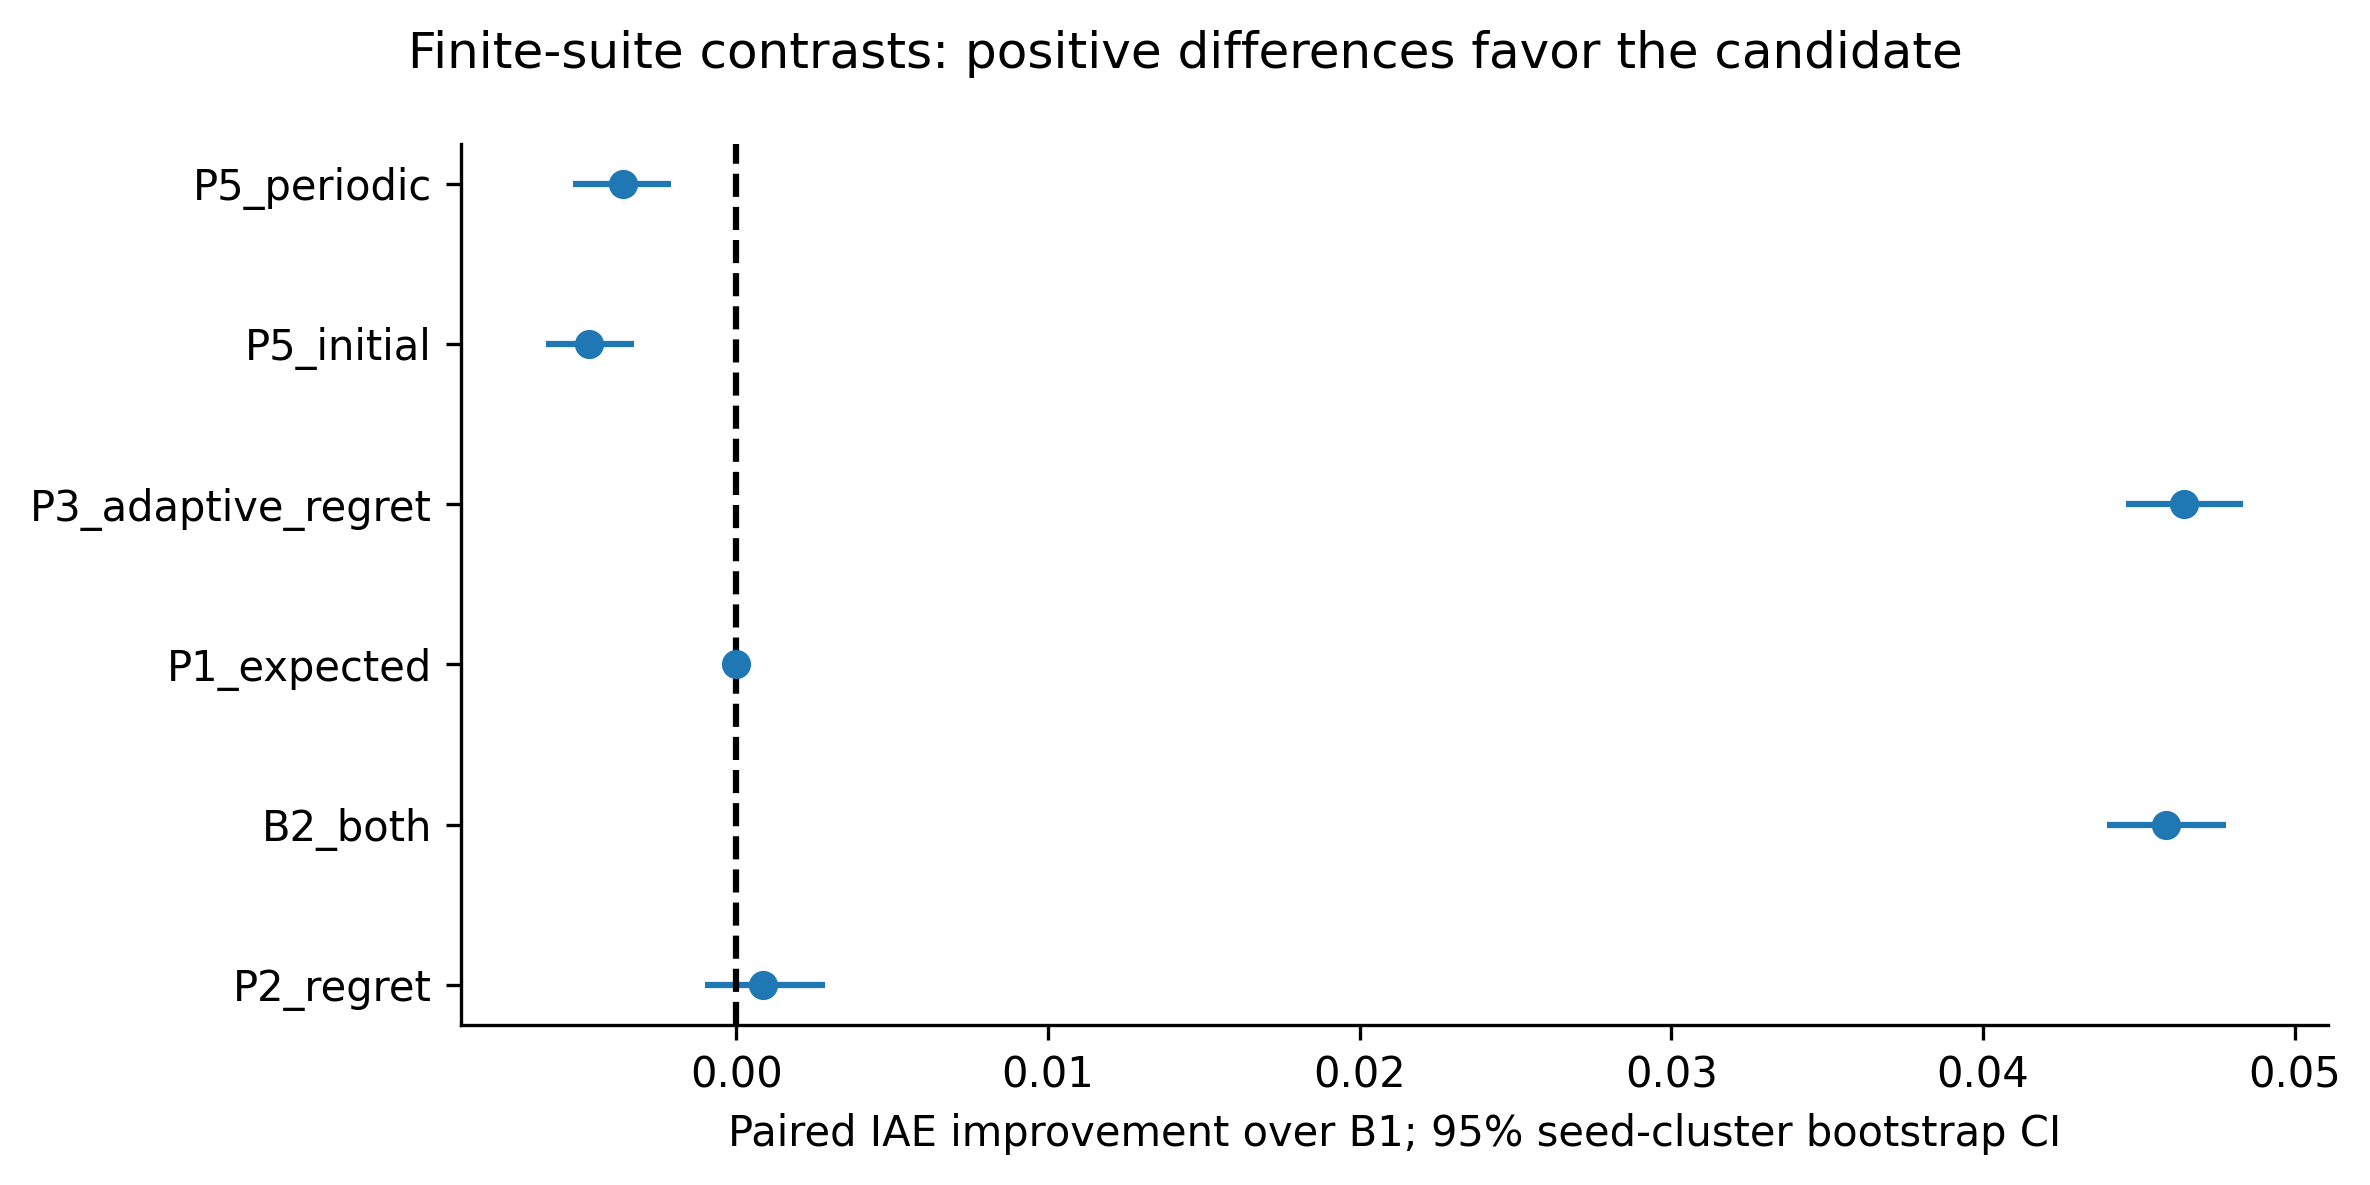
\includegraphics{figures/Figure_13.png}
\caption{Figure 13. Finite-suite contrasts: positive differences favor
the candidate}
\end{figure}

\begin{figure}
\centering
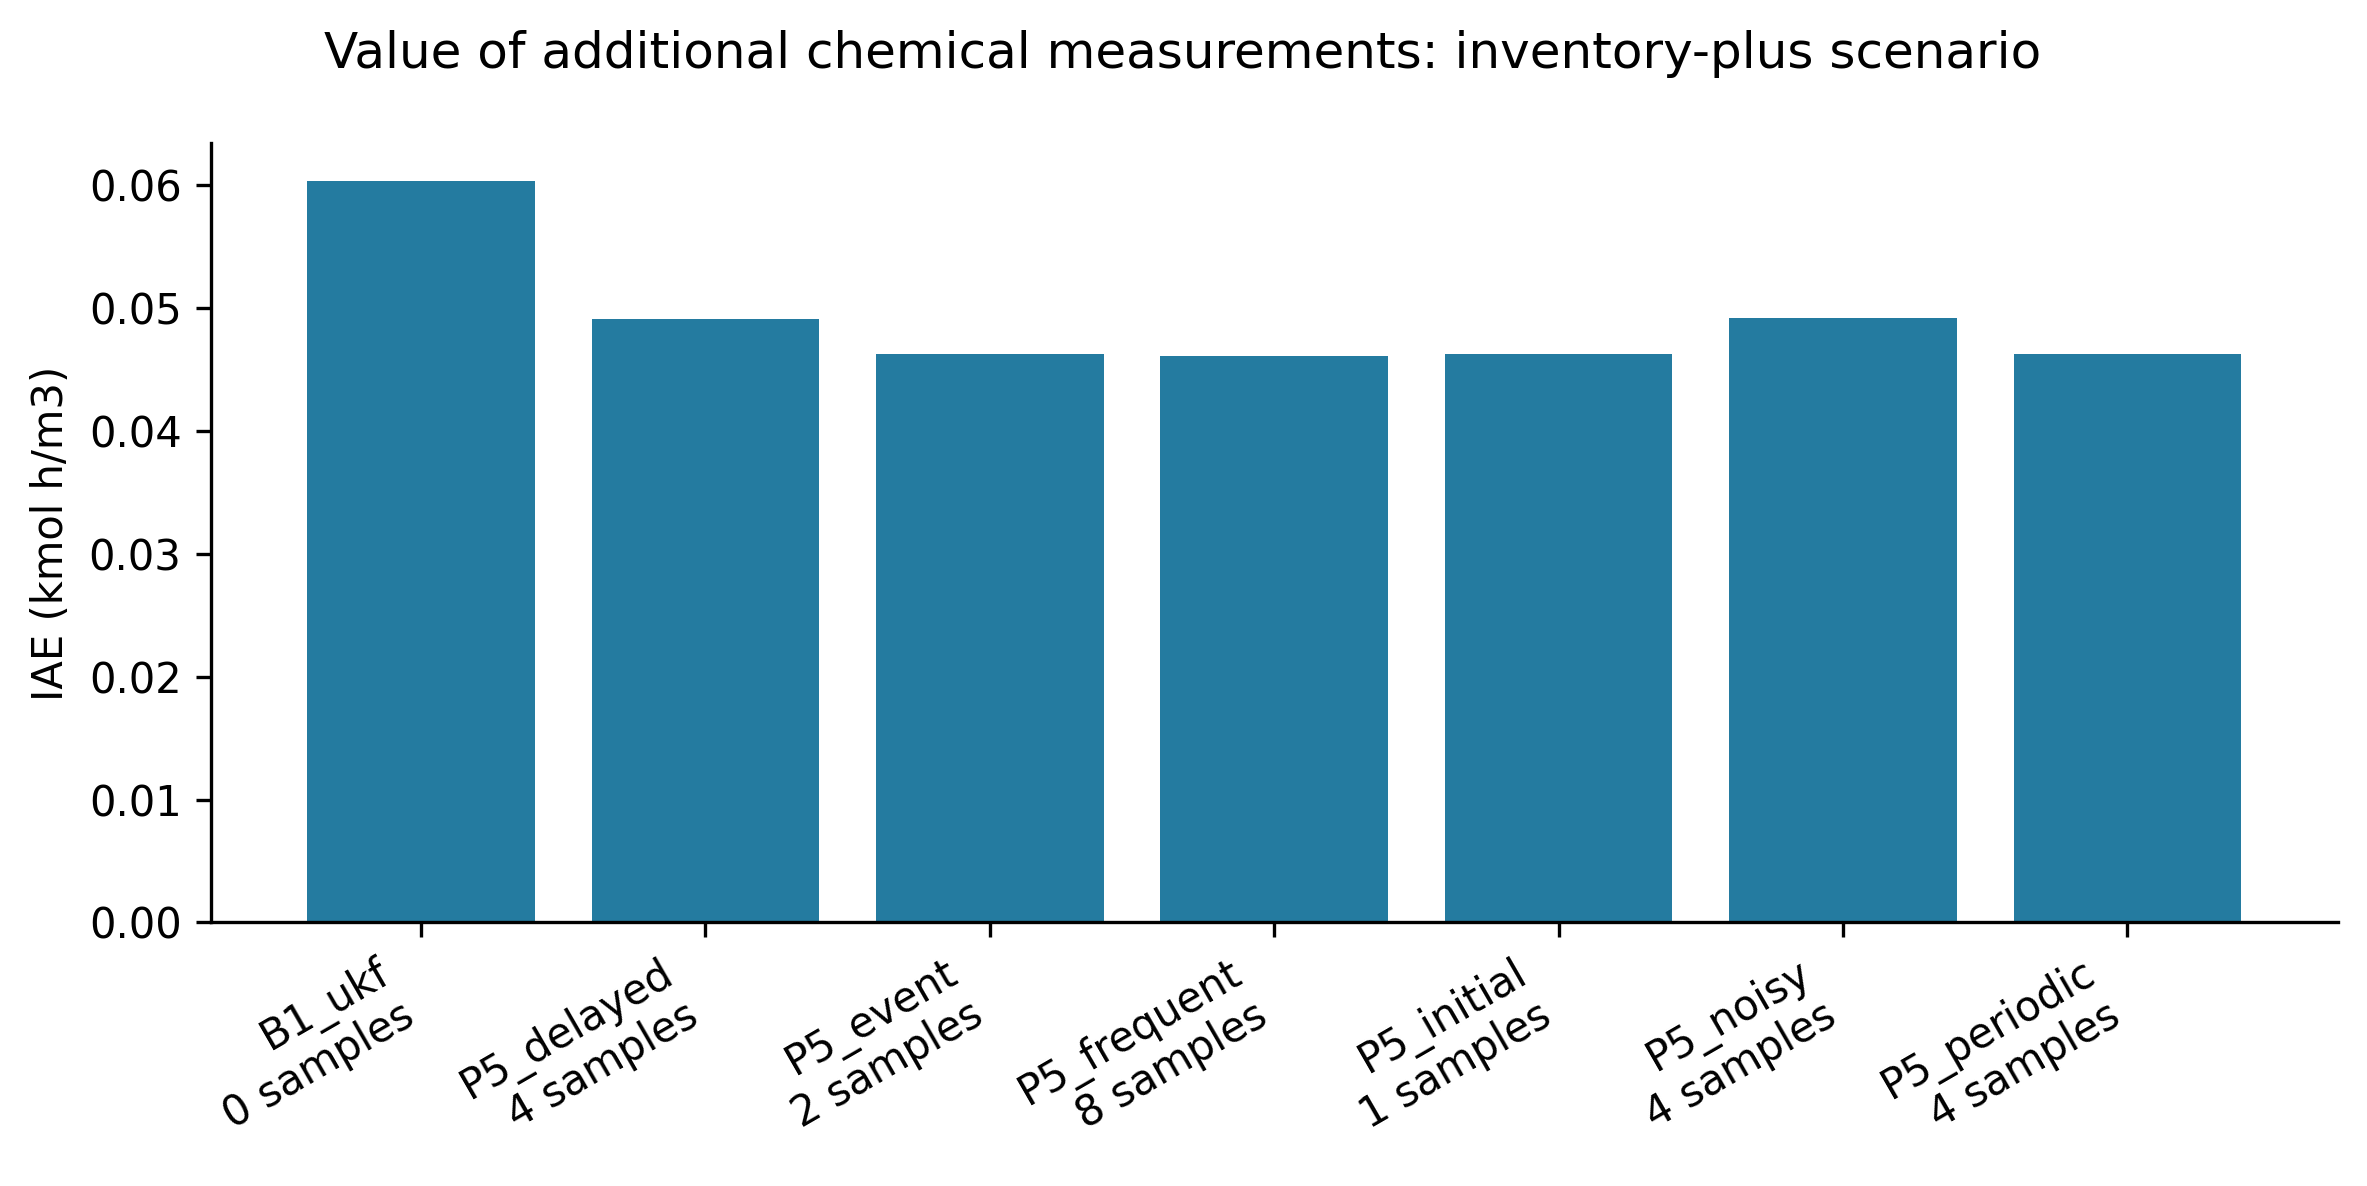
\includegraphics{figures/Figure_14.png}
\caption{Figure 14. Value of additional chemical measurements:
inventory-plus scenario}
\end{figure}

\begin{figure}
\centering
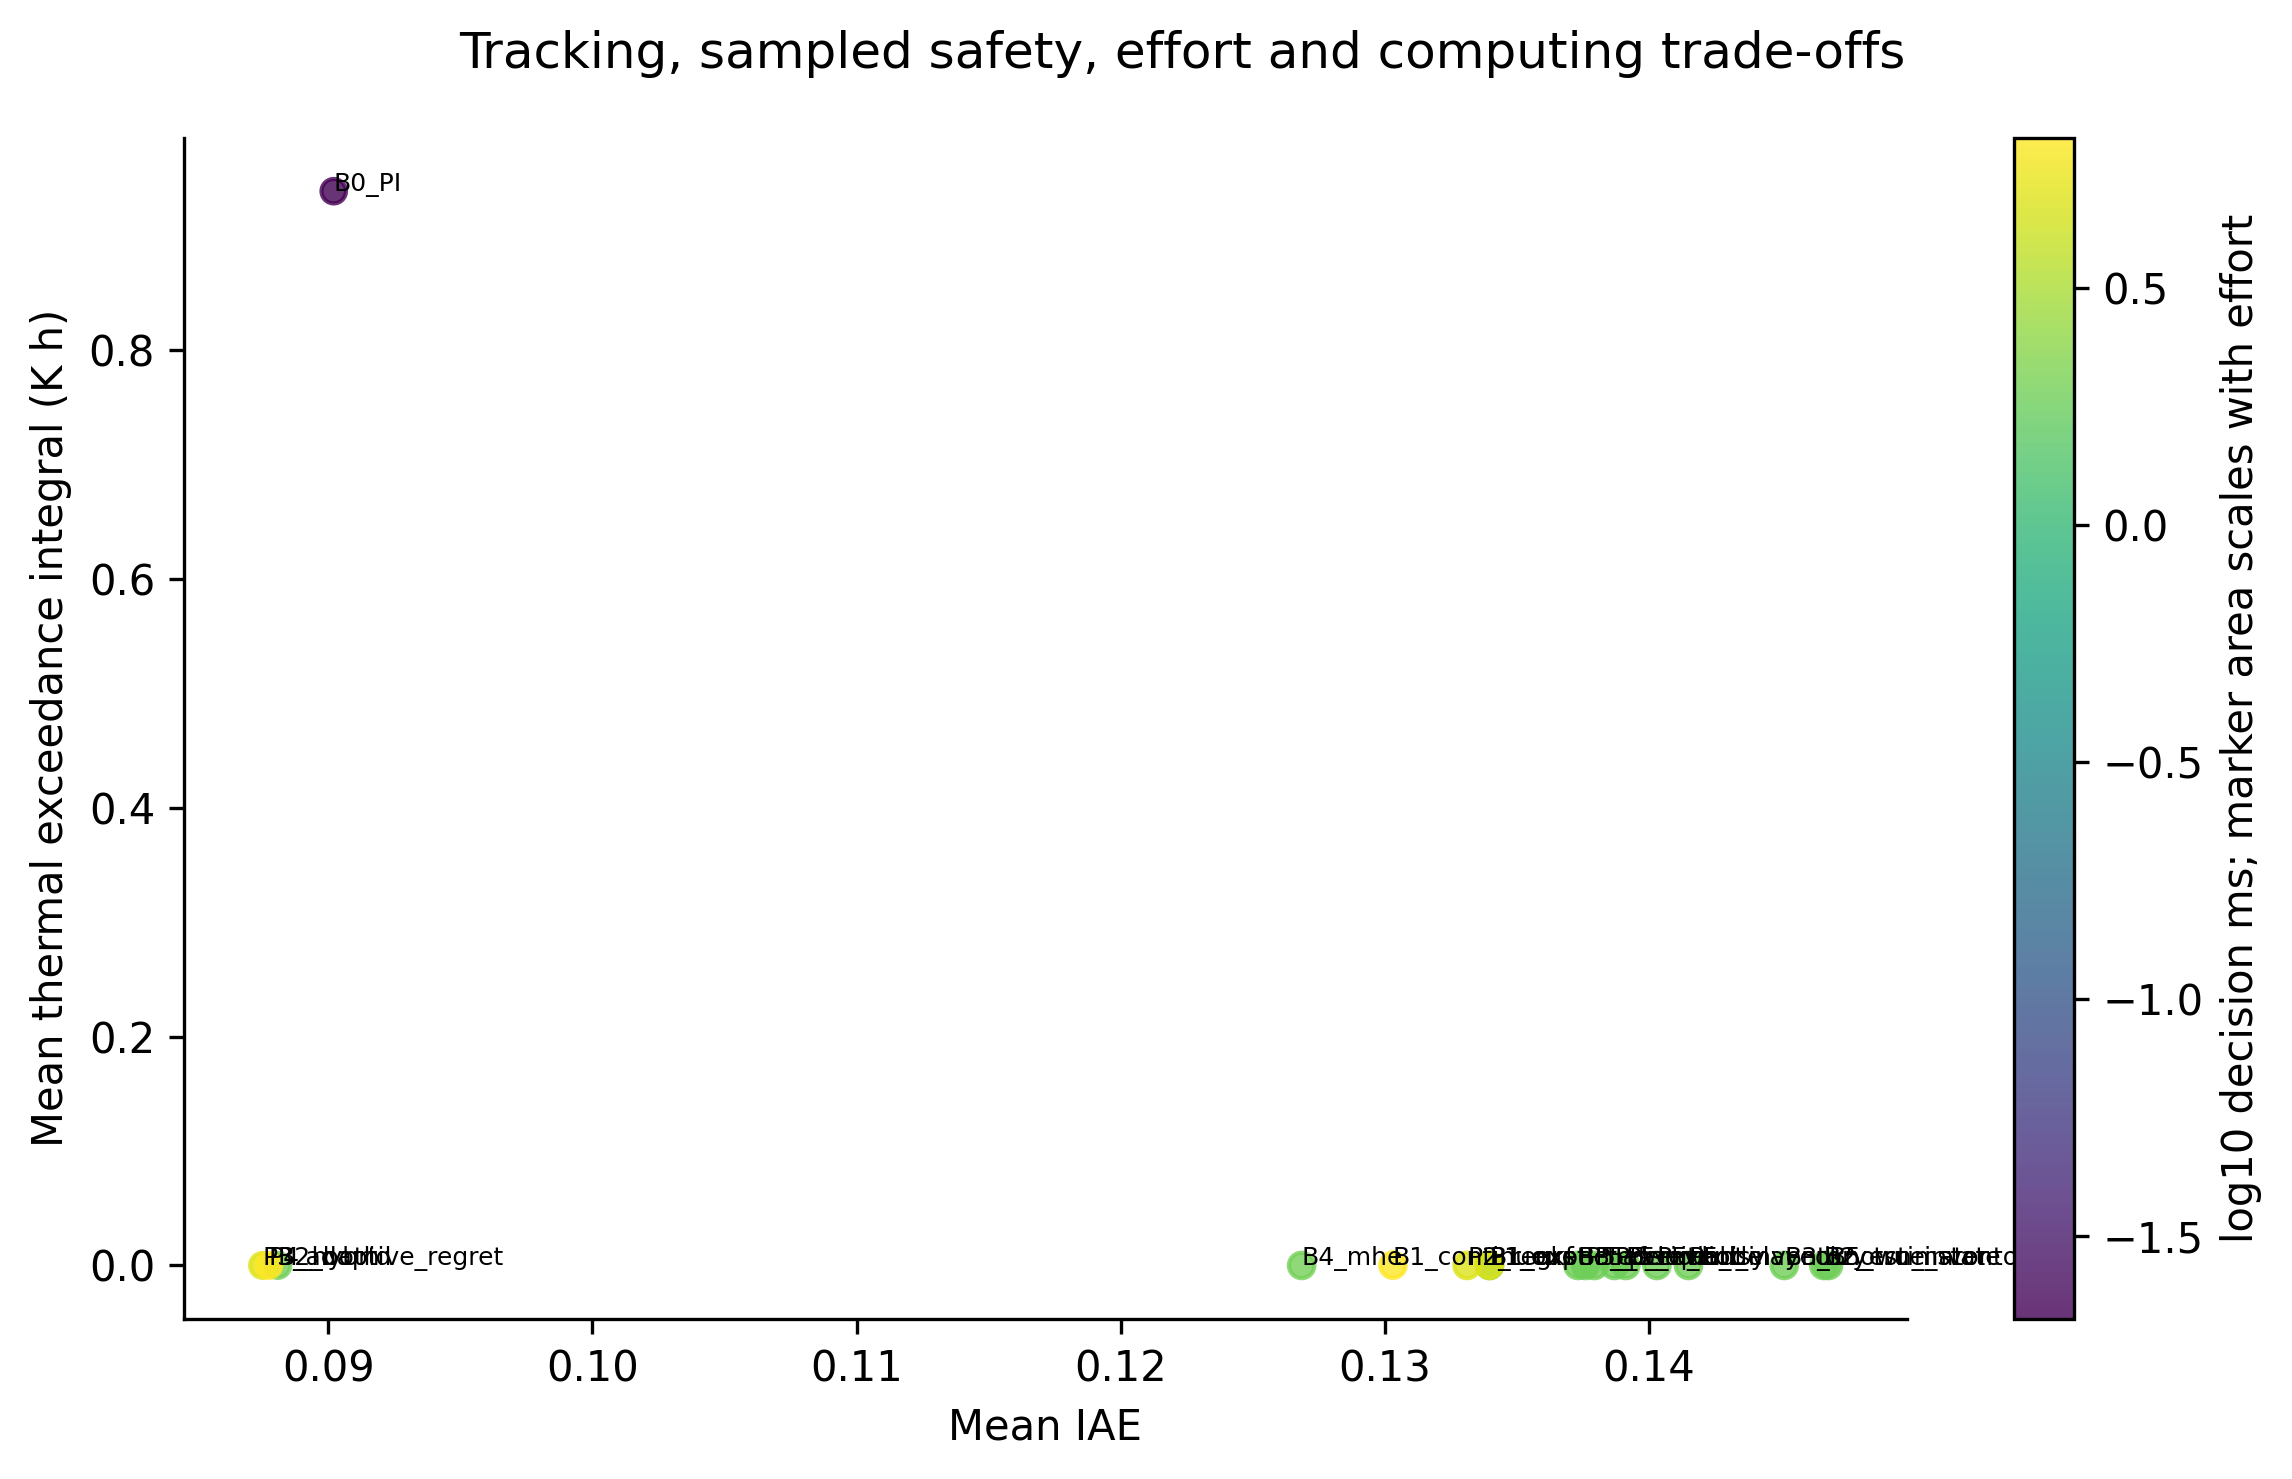
\includegraphics{figures/Figure_15.png}
\caption{Figure 15. Tracking, sampled safety, effort and computing
trade-offs}
\end{figure}

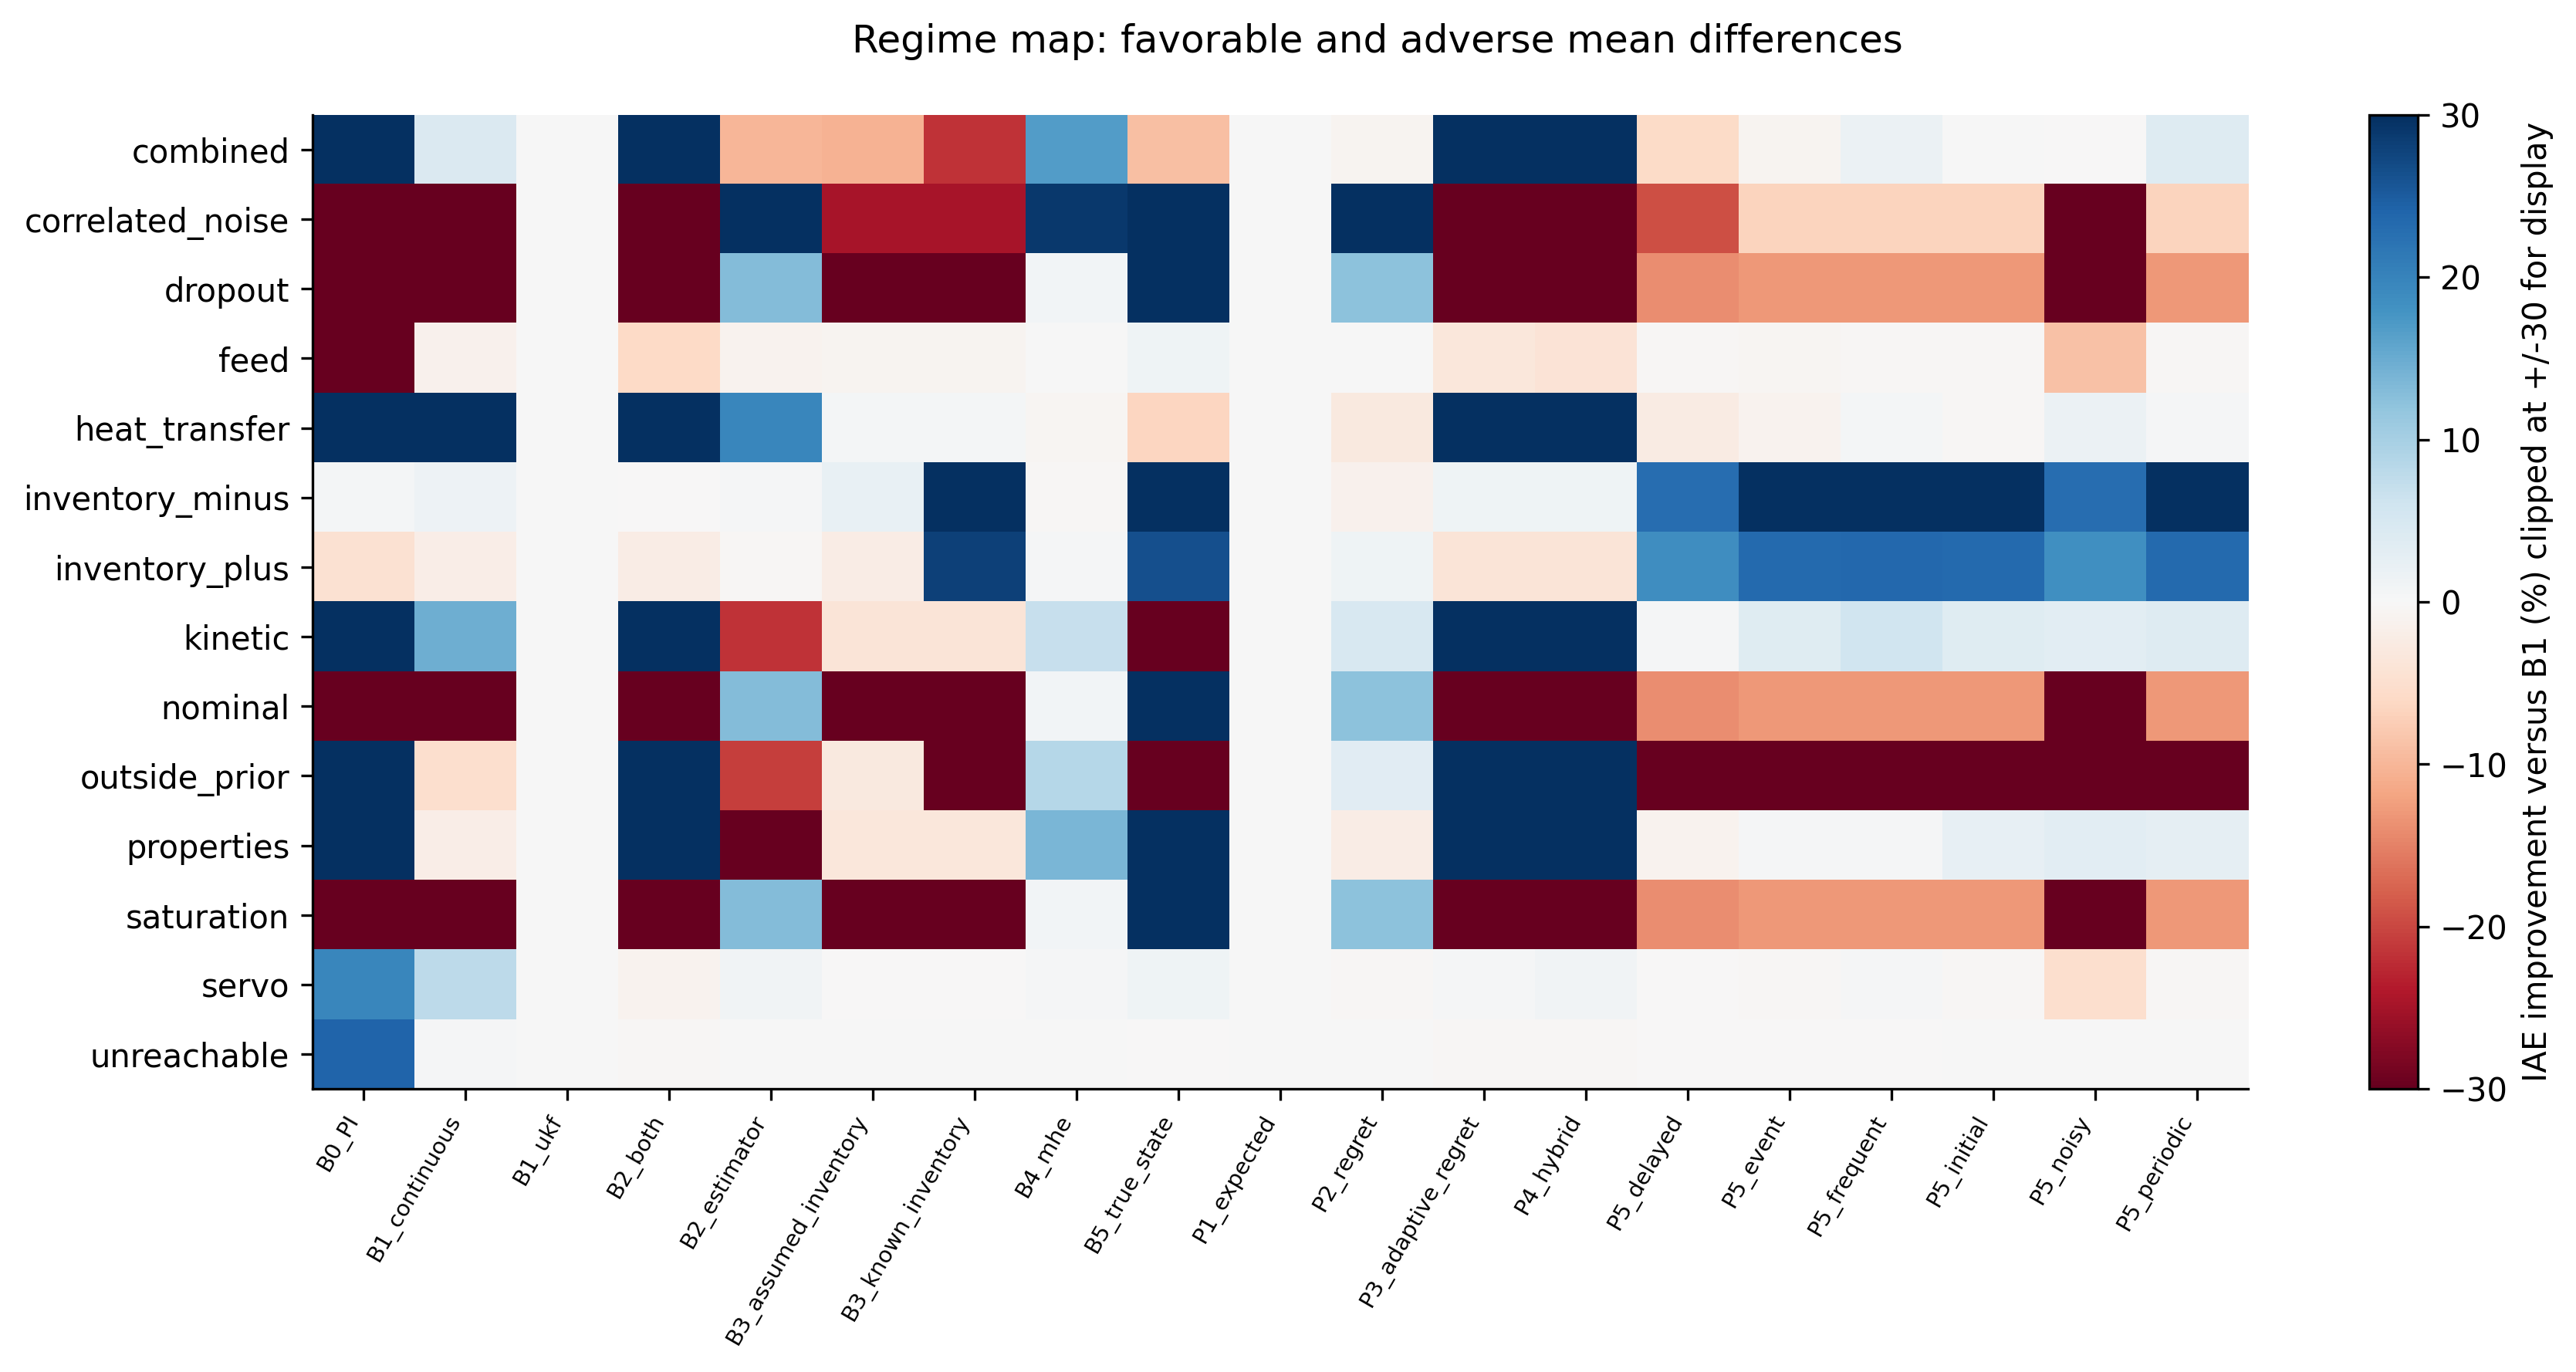
\includegraphics{figures/Figure_16.png} \# References

\hypertarget{refs}{}
\begin{CSLReferences}{1}{0}
\leavevmode\vadjust pre{\hypertarget{ref-brandao2019}{}}%
Brandao, Walter Yanko de Aragao. 2019. {``Uso de Observadores de Estado
Aplicados No Controle Inferencial Preditivo de Processos Nao
Lineares.''} Master's thesis, Universidade Federal de Campina Grande.
\url{https://dspace.sti.ufcg.edu.br/handle/riufcg/12684}.

\leavevmode\vadjust pre{\hypertarget{ref-cao2026}{}}%
Cao, Daniel, Beixi Du, Andrew Lowitt, Sunmook Choi, Sarah Dean, and
Yahya Sattar. 2026. {``Dual Control of Linear Systems from Bilinear
Observations with Belief Space Model Predictive Control.''}
\url{https://arxiv.org/abs/2604.24663}.

\leavevmode\vadjust pre{\hypertarget{ref-chan2004}{}}%
Chan, Arthur, and Warren D. Seider. 2004. {``Batch Manufacture of
Propylene Glycol.''} University of Pennsylvania.
\url{https://www.engineering.upenn.edu/~dlewin/CACHE_Workshop/Batch\%20Manufacture\%20of\%20Propylene\%20Glycol.pdf}.

\leavevmode\vadjust pre{\hypertarget{ref-elmachtoub2022}{}}%
Elmachtoub, Adam N., and Paul Grigas. 2022. {``Smart {Predict, then
Optimize}.''} \emph{Management Science} 68 (1): 9--26.
\url{https://doi.org/10.1287/mnsc.2020.3922}.

\leavevmode\vadjust pre{\hypertarget{ref-enwerem2026}{}}%
Enwerem, Clinton, John S. Baras, and Calin Belta. 2026.
{``Risk-Constrained Belief-Space Optimization for Safe Control Under
Latent Uncertainty.''} \url{https://arxiv.org/abs/2604.03868}.

\leavevmode\vadjust pre{\hypertarget{ref-fogler_examples}{}}%
Fogler, H. Scott. n.d. {``Elements of Chemical Reaction Engineering:
Sixth-Edition Living Examples, Chapter 12.''} University of Michigan
teaching resources.
\url{https://public.websites.umich.edu/~elements/6e/12chap/live.html}.

\leavevmode\vadjust pre{\hypertarget{ref-goel2021}{}}%
Goel, Gautam, and Babak Hassibi. 2021. {``Regret-Optimal
Measurement-Feedback Control.''} In \emph{Proceedings of the 3rd
Conference on Learning for Dynamics and Control}, 144:1270--80.
Proceedings of Machine Learning Research.
\url{https://proceedings.mlr.press/v144/goel21a.html}.

\leavevmode\vadjust pre{\hypertarget{ref-hermann1977}{}}%
Hermann, Robert, and Arthur J. Krener. 1977. {``Nonlinear
Controllability and Observability.''} \emph{IEEE Transactions on
Automatic Control} 22 (5): 728--40.
\url{https://doi.org/10.1109/TAC.1977.1101601}.

\leavevmode\vadjust pre{\hypertarget{ref-klenske2016}{}}%
Klenske, Edgar D., and Philipp Hennig. 2016. {``Dual Control for
Approximate Bayesian Reinforcement Learning.''} \emph{Journal of Machine
Learning Research} 17 (127): 1--30.
\url{https://www.jmlr.org/papers/v17/15-162.html}.

\leavevmode\vadjust pre{\hypertarget{ref-lall2002}{}}%
Lall, Sanjay, Jerrold E. Marsden, and Sonja Glavaski. 2002. {``A
Subspace Approach to Balanced Truncation for Model Reduction of
Nonlinear Control Systems.''} \emph{International Journal of Robust and
Nonlinear Control} 12: 519--35. \url{https://doi.org/10.1002/rnc.657}.

\leavevmode\vadjust pre{\hypertarget{ref-rao2003}{}}%
Rao, Christopher V., James B. Rawlings, and David Q. Mayne. 2003.
{``Constrained State Estimation for Nonlinear Discrete-Time Systems:
Stability and Moving Horizon Approximations.''} \emph{IEEE Transactions
on Automatic Control} 48 (2): 246--58.
\url{https://doi.org/10.1109/TAC.2002.808470}.

\leavevmode\vadjust pre{\hypertarget{ref-rawlings2017}{}}%
Rawlings, James B., David Q. Mayne, and Moritz M. Diehl. 2017.
\emph{Model Predictive Control: Theory, Computation, and Design}. 2nd
ed. Nob Hill Publishing.
\url{https://sites.chemengr.ucsb.edu/~jbraw/mpc/}.

\leavevmode\vadjust pre{\hypertarget{ref-schaum2007}{}}%
Schaum, Alexander, Jaime A. Moreno, Jorge Diaz-Salgado, and Jesus
Alvarez. 2007. {``Dissipativity-Based Observer and Feedback Control
Design for a Class of Chemical Reactors.''} In \emph{8th IFAC Symposium
on Dynamics and Control of Process Systems}.
\url{https://skoge.folk.ntnu.no/prost/proceedings/dycops2007-and-cab2007/DYCOPS/Friday/DissipativityBasedControl/V32_291_Paper_stamped_noAS.pdf}.

\leavevmode\vadjust pre{\hypertarget{ref-villaverde2016}{}}%
Villaverde, Alejandro F., Antonio Barreiro, and Antonis
Papachristodoulou. 2016. {``Structural Identifiability of Dynamic
Systems Biology Models.''} \emph{PLoS Computational Biology} 12 (10):
e1005153. \url{https://doi.org/10.1371/journal.pcbi.1005153}.

\end{CSLReferences}

\end{document}
